\appendix
\chapter{Appendices}
% \addcontentsline{toc}{chapter}{Appendices}
\section{Repository Information}

The code for this project is located in the GitLab repository \\\href{https://git.cs.bham.ac.uk/projects-2023-24/oxg397}{https://git.cs.bham.ac.uk/projects-2023-24/oxg397}

\subsubsection{Installation} 
To set up the environment and install the required packages, run:

\begin{verbatim}
conda create -y --name final-project python=3.10
conda activate final-project
pip install torchrl torch torchvision torchviz wandb
pip install hydra-core tqdm gymnasium gymnasium[classic-control]
\end{verbatim}

\textbf{Disclaimer}: there could be incompatible issues due to the nvidia driver versions, we recommend to set \texttt{device: cpu} in the configuration file for running using the cpu.

\subsubsection{Usage}

\begin{enumerate}
    \item \textbf{Run Training}: Open a folder with \texttt{dqn\_<something>/} and run the main script \texttt{python dqn\_<something>.py} to start training.
    \item \textbf{Monitor Training}: Track the training progress using \texttt{wandb} or any other configured visualization tool. The \texttt{wandb} is disabled by default.
\end{enumerate}

\subsubsection{Repository Structure} 
The algorithms were divided into different folders for easy implementation and changes.

\begin{itemize}
    \item \textbf{\texttt{dqn\_gridworld/}}: Contains implementations of various DQN variants for grid-based environments:
    \begin{itemize}
        \item \textbf{Variants Included}: DQN, DQN + MICO, DQN + PER, DQN + MICO + BPERcn, and DQN + MICO + BPERaa.
        \item \textbf{Customization}: Hyperparameters are configurable through \texttt{config\_gridworld.yaml}.
        \item \textbf{Files:}
        \begin{itemize}
            \item \texttt{dqn.py}: Main reinforcement learning loop.
            \item \texttt{utils\_experiments.py}: Additional functions for conducting and managing experiments.
            \item \texttt{utils\_grid\_world.py}: Functions related to customizing the grid world environment in TorchRL.
            \item \texttt{utils\_metric.py}: Functions to calculate the MICo bisimulation metric, based on \href{https://github.com/google-research/google-research/blob/master/mico/atari/metric_utils.py}{Google Research MICO}.
            \item \texttt{utils\_modules.py}: Definitions of customized models, such as the DQN with MICO loss and DQN network with representation outputs.
        \end{itemize}
    \end{itemize}

    \item \textbf{\texttt{dqn\_pixel/}}: Implements DQN and DQN + PER variants for pixel-based environments:
    \begin{itemize}
        \item \textbf{Customization}: Configurable through \texttt{config.yaml}.
        \item \textbf{Files:}
        \begin{itemize}
            \item \texttt{utils\_dqn.py}: Functions related to customization for pixel-based environments in TorchRL.
            \item \texttt{utils\_modules.py}: Definitions of customized models for pixel-based DQN variants.
        \end{itemize}
    \end{itemize}

    \item \textbf{\texttt{dqn\_pixel\_mico/}}: Implements DQN variants using MICO for pixel environments:
    \begin{itemize}
        \item \textbf{Variants Included}: DQN + MICO, DQN + MICO + BPERcn, and DQN + MICO + BPERaa.
        \item \textbf{Customization}: Configurable through \texttt{config.yaml}.
        \item \textbf{Files:}
        \begin{itemize}
            \item \texttt{utils\_dqn.py}: Functions related to customization for pixel-based environments in TorchRL.
            \item \texttt{utils\_modules.py}: Definitions of customized models.
            \item \texttt{utils\_metric.py}: Functions to calculate the MICo bisimulation metric, similar to \href{https://github.com/google-research/google-research/blob/master/mico/atari/metric_utils.py}{Google Research MICO}.
        \end{itemize}
    \end{itemize}

    \item \textbf{\texttt{motivating\_example/}}: Contains notebooks for calculating exact bisimulation, on-policy bisimulation, bisimulation metric, and on-policy bisimulation metric using the Grid World environment.

    \item \textbf{\texttt{plot\_utils/}}: Contains notebooks for generating and customizing plots of experiment results.

    \item \textbf{\texttt{custom\_envs/}}: Contains proposed Grid World environments defined in \texttt{.txt} files and the \texttt{GridWorld} class to set up these environments in Gym.

    \item \textbf{Miscellaneous}:
    \begin{itemize}
        \item Sandboxes and notebooks scattered throughout the repository were used for testing small features but are no longer relevant.
    \end{itemize}
\end{itemize}


% \section{Metrics}
% \label{append:metrics}

% The following information was retrieved from the Supplementary Material provide by Castro et al. \cite{castro2021mico}. 

% A \textbf{metric} \(d\) on a set \(X\) is a function \(d : X \times X \to [0, \infty)\) respecting the following axioms for any \(x, y, z \in X\):

% \begin{enumerate}
%     \item \textbf{Identity of indiscernibles:} \(d(x, y) = 0 \iff x = y\);
%     \item \textbf{Symmetry:} \(d(x, y) = d(y, x)\);
%     \item \textbf{Triangle inequality:} \(d(x, y) \leq d(x, z) + d(z, y)\).
% \end{enumerate}

% A \textbf{pseudometric} is similar, but the "identity of indiscernibles" axiom is weakened:

% \begin{enumerate}
%     \item \(x = y \implies d(x, y) = 0\);
%     \item \(d(x, y) = d(y, x)\);
%     \item \(d(x, y) \leq d(x, z) + d(z, y)\).
% \end{enumerate}

% Note that the weakened first condition \emph{does} allow one to have \(d(x, y) = 0\) when \(x \neq y\).

% A \textbf{(pseudo)metric space} \((X, d)\) is defined as a set \(X\) together with a (pseudo)metric \(d\) defined on \(X\).

% A \textbf{diffuse metric} is similar to as pseudometri, but the 'identity of indiscernibles' axiom is weakened even more:

% \begin{enumerate}
%     \item \(d(x, y) \geq 0\) for any $x, y \in X$;
%     \item \(d(x, y) = d(y, x)\);
%     \item \(d(x, y) \leq d(x, z) + d(z, y)\).
% \end{enumerate}

% Note that the weakened first condition \emph{does} allow one to have self-distance greater than zero $d(x,x) > 0$.

% \section{Algorithm: DQN with Matching under Independent Couplings (MICo)}
% \label{append:dqn_mico}

% \begin{algorithm}[H]
% \caption{DQN with Matching under Independent Couplings (MICo)}
% \label{algorithm:dqn_mico}
% \begin{algorithmic}[1]
% \State \textbf{Input:} minibatch $k$, step-size $\eta$, replay period $K$ and size $N$, budget $T$ (total steps).
% \State \textbf{Initialize} action-value function $Q$ with random weights $\xi$, $\omega$
% \State \textbf{Initialize} target action-value function $Q^-$ with weights $\{\bar{\xi},\bar{\omega}\} \leftarrow \{\xi, \omega\}$
% \State \textbf{Initialize} replay memory $\mathcal{D} = \emptyset$ with capacity $N$%$\Delta_{\{\xi, \omega\}} = 0$, $\Delta_\omega = 0$, $p_1 = 1$
% % \State Observe $s_0$ and choose $a_0 \sim \pi^\epsilon_\theta(s_0)$ 
% \For{$t = 1$ to $T$}
%     \State Observe $s_t$
%     \State Choose action $a_t \sim \pi^\epsilon_\theta(s_t)$
%     \State Execute action $a_t$ and observe $r_t$ and $s_{t+1}$
%     \State Store transition $(s_t, a_t, r_t, s_{t+1})$ in $\mathcal{D}$
%     \If{$t \equiv 0 \mod K$}
%         % \For{$j = 1$ to $k$}
%         \State Sample minibatch $B \sim \text{Uniform}(\mathcal{D})$ of transitions $e_j$        % \State Compute importance-sampling weight $w_j = \left( N \cdot P(j) \right)^{-\beta} / \max_i w_i$
%         \State Set $y_j = 
%         \begin{cases} 
%             r_j & \text{for terminal } s_{j+1}\\
%             r_j + \gamma \max_{a'} Q^-(s_{j+1}, a'; \{\bar{\xi},\bar{\omega}\}) & \text{otherwise}
%         \end{cases}$
%         \State Compute TD-error $\delta_j = y_j - Q(s_{j}, a_{j}; \{\xi, \omega\})$, and loss $\mathcal{L}_{\text{TD}} = \delta_j^2 $
%         \State Squarify minibatch $B$ to get transition pairs $\left\langle x, r_x, x^{\prime}\right\rangle,\left\langle y, r_y, y^{\prime}\right\rangle$ 
%         \State Compute MICo loss $\mathcal{L}_{\text{MICo}} = \left(T_{\bar{\omega}}^U\left(r_x, x^{\prime}, r_y, y^{\prime}\right)-U_\omega(x, y)\right)^2$
%         \State Compute total loss $\mathcal{L}_\alpha(\xi, \omega) = (1 - \alpha) \mathcal{L}_{\text{TD}}(\xi, \omega) + \alpha \mathcal{L}_{\text{MICo}}(\omega)$
%         \State Perform a gradient descent step on $\mathcal{L}_\alpha(\xi, \omega)$
%         % \State Update transition priority $p_j \leftarrow (1 - \mu) |\delta_j| + \mu U_\omega(s_j,s_{j+1}) + \epsilon$
%         \State Every C optimizing steps update $\{\bar{\xi},\bar{\omega}\} \leftarrow \{\xi, \omega\}$
        

        
%         % \State Accumulate weight-change $\Delta_{\{\xi, \omega\}} \leftarrow \Delta_{\{\xi, \omega\}} + w_j \cdot \delta_j \cdot \nabla_\theta Q(s_{j}, a_{j})$
%         % \State Compute bisimulation distance error $\sigma_j = T_{\bar{\omega}}^U\left(r_x, x^{\prime}, r_y, y^{\prime}\right)-U_\omega(x, y)$
%         %  \State Accumulate weight-change $\Delta_{\omega} \leftarrow \Delta_{\omega} + w_j \cdot \sigma_j \cdot \nabla_\omega U_\omega(s_{i}, a_{j})$   

%         % \EndFor
%         % \State Update weights $\theta \leftarrow \theta + \eta \cdot \Delta$, reset $\Delta = 0$
%     \EndIf
% \EndFor
% \end{algorithmic}
% \end{algorithm}

% \newpage
% \section{Distance between Priority Sampling Distributions}
% \label{append:distance_distributions}

% The following explanation is based on the Supplementary Materials from Pan et al. \cite{pan2022understanding}. The distance between the ideal priority distribution $p^\ast_i(\cdot)$ and the sampling priority distribution $p^\ast_i(\cdot)$ is estimated by the following three steps: 

% \begin{enumerate}
%     \item In order to compute the ideal sampling distribution, we use the implicit discrete state space (not raw pixels) from the Grid World, and
%     \begin{itemize}
%         \item In the DQN + PER experiment, we calculate the absolute TD error of each state (coordinates $x,y$) by using the true environment model and \textbf{the current learned $Q_{\{\xi,\omega\}}$ network}.
%         \item In the DQN + MICO + PER experiment, we calculate the mico distance of each state (coordinates $x,y$) by using the true environement model and \textbf{the current learned $\phi_{\omega}$ encoder}
%     \end{itemize}
%     We then normalize these priorities to get probability distribution \(p^*_i\) with $i=1$ for DQN + PER and $i=2$ for DQN + MICO + PER. Note that this distribution is considered as the desired one since we have access to all states across the state space with priorities computed by current network at each time step.

%     \item The sampling distribution is estimated by randomly sampling 3k states and count the number of states and normalize these counts to get \(p_i\), with $i=1$ for DQN + PER and $i=2$ for DQN + MICO + PER.

%     \item Finally, the distances of \(p_1, p_2\) to \(p^*_1,p^*_2\) by two weighting schemes: 

%     \begin{enumerate}
%         \item \textbf{on-policy weighting}: 
%             \[
%             \sum_{j=1}^{2500} d^{\pi}(s_j) |p_i(s_j) - p^*_i(s_j)|, \quad i \in \{1, 2\},
%             \]
%         where \(d^{\pi}\) is approximated by uniformly sampling 3k states from a recent buffer and normalizing their visitation counts on the GridWorld;
%         \item  \textbf{uniform weighting}:
%     \[
%     \frac{1}{2500} \sum_{j=1}^{2500} |p_i(s_j) - p^*_i(s_j)|, \quad i \in \{1, 2\}.
%     \]
%     \end{enumerate}
    
% \end{enumerate}

% Two weighting schemes were employed for two different purposes: \textbf{on-policy weighting} focuses on the asymptotic convergence behavior, thereby reducing the weight of states with relatively high TD errors that are rarely visited as the policy approaches optimality. In contrast, \textbf{uniform weighting} is more appropriate during the initial learning phase, where all states are considered equally important, encouraging the agents to thoroughly explore the entire state space.



% % Given the sampling distribution of priorities pi(·) from the experience buffer and
% % the corresponding ideal distribution p
% % ∗
% % i
% % (·) (theoretically achieved when all state
% % space priorities are updated at each time step7
% % ), 1) the on-policy weighting is
% % given by P31
% % j=1 w
% % π
% % (sj )|pi(sj ) − p
% % ∗
% % i
% % (sj )|, i ∈ {1, 2}, and 2) the uniform weighting is
% % 1
% % 31
% % P31
% % j=1 |pi(sj ) − p
% % ∗
% % i
% % (sj )|, i ∈ {1, 2}, where p1 corresponds to the PER method and
% % p2 corresponds to the BPER method. A more detailed explanation of this procedure
% % is provided in the Appendix ??.

% \section{Hyperparameters Setting}
% \label{append:hyperparameters}

% \begin{table}[H]
% \centering

% \hspace*{-1cm}
% \begin{tabular}{@{} lccccc @{}}
% \toprule
% & \textbf{Hyperparameter} & {\footnotesize\textbf{DQN}} & {\footnotesize \textbf{DQN PER}} & {\footnotesize\textbf{DQN MICo}} & {\footnotesize\textbf{DQN BPER}} \\ 
% \midrule

% \multirow{8}{*}{\textbf{Collector}} 
% & Total Budget & 100,000 & 100,000 & 100,000 & 100,000 \\ 
% & Replay Period & 128 & 128 & 128 & 128 \\ 
% & Eps Start & 0.1 & 0.1 & 0.1 & 0.1 \\ 
% & Eps End & 0.005 & 0.005 & 0.005 & 0.005 \\ 
% & Eps Annealing Frames & 520,000 & 520,000 & 520,000 & 520,000 \\ 
% & Init Random Frames & 200 & 200 & 200 & 200 \\ 
% & Frame Stack & 1 & 1 & 1 & 1 \\
% & Frame Skip & 1 & 1 & 1 & 1 \\ 
% \midrule

% \multirow{5}{*}{\textbf{Policy}} 
% & CNN Net (Cells) & [32, 64, 64] & [32, 64, 64] & [32, 64, 64] & [32, 64, 64] \\ 
% & Kernel Sizes & [8, 4, 3] & [8, 4, 3] & [8, 4, 3] & [8, 4, 3] \\ 
% & Strides & [4, 2, 1] & [4, 2, 1] & [4, 2, 1] & [4, 2, 1] \\ 
% & MLP Net (Cells) & [64, 64] & [64, 64] & [64, 64] & [64, 64] \\ 
% & Activation & ReLU & ReLU & ReLU & ReLU \\ 
% \midrule

% \multirow{5}{*}{\textbf{Buffer}} 
% & Buffer Size & 100,000 & 100,000 & 100,000 & 100,000 \\ 
% & Batch Size & 256 & 256 & 256 & 256 \\ 
% & Alpha & -- & 0.6 & -- & 0.6 \\ 
% & Beta & -- & 0.4 & -- & 0.4 \\ 
% & Priority Weight & -- & -- & 1.0 & 1.0 \\ 
% \midrule

% \multirow{4}{*}{\textbf{Optim}} 
% & Learning Rate & 0.0015 & 0.0015 & 0.0015 & 0.0015 \\ 
% & Max Grad Norm & 10 & 10 & 10 & 10 \\ 
% & Weight Decay & 0.00001 & 0.00001 & 0.00001 & 0.00001 \\ 
% & Eps & 1.5e-4 & 1.5e-4 & 1.5e-4 & 1.5e-4 \\ 
% \midrule

% \multirow{6}{*}{\textbf{Loss}} 
% & Gamma & 0.99 & 0.99 & 0.99 & 0.99 \\ 
% & MICO Weight & -- & -- & 0.01 & 0.01 \\ 
% & MICO Beta & -- & -- & 0.1 & 0.1 \\ 
% & MICO Gamma & -- & -- & 0.99 & 0.99 \\ 
% & Hard Update Freq & 50 & 50 & 50 & 50 \\ 
% & Num Updates & 1 & 1 & 1 & 1 \\ 
% \bottomrule

% \end{tabular}
% \caption[Hyperparameter Configurations for Grid World]{\textbf{Hyperparameter Configurations for Grid World.} This configuration was consistently used across different independent runs. The settings for DQN BPER are applicable to both BPERcn and BPERaa.}
% \end{table}

% \begin{table}[H]
% \centering

% \hspace*{-1cm}
% \begin{tabular}{@{} lccccc @{}}
% \toprule
% & \textbf{Hyperparameter} & {\footnotesize\textbf{DQN}} & {\footnotesize \textbf{DQN PER}} & {\footnotesize\textbf{DQN MICo}} & {\footnotesize\textbf{DQN BPER}} \\ 
% \midrule

% \multirow{8}{*}{\textbf{Collector}} 
% & Total Budget & 1,000,064 & 1,000,064 & 1,000,064 & 1,000,064 \\ 
% & Replay Period & 128 & 128 & 128 & 128 \\ 
% & Eps Start & 0.5 & 0.5 & 0.5 & 0.5 \\ 
% & Eps End & 0.005 & 0.005 & 0.005 & 0.005 \\ 
% & Eps Annealing Frames & 520,000 & 520,000 & 520,000 & 520,000 \\ 
% & Init Random Frames & 20,000 & 20,000 & 20,000 & 20,000 \\ 
% & Frame Stack & 4 & 4 & 4 & 4 \\
% & Frame Skip & 4 & 4 & 4 & 4 \\ 
% \midrule

% \multirow{5}{*}{\textbf{Policy}} 
% & CNN Net (Cells) & [32, 64, 64] & [32, 64, 64] & [32, 64, 64] & [32, 64, 64] \\ 
% & Kernel Sizes & [8, 4, 3] & [8, 4, 3] & [8, 4, 3] & [8, 4, 3] \\ 
% & Strides & [4, 2, 1] & [4, 2, 1] & [4, 2, 1] & [4, 2, 1] \\ 
% & MLP Net (Cells) & [64, 64] & [64, 64] & [64, 64] & [64, 64] \\ 
% & Activation & ReLU & ReLU & ReLU & ReLU \\ 
% \midrule

% \multirow{5}{*}{\textbf{Buffer}} 
% & Buffer Size & 100,000 & 100,000 & 100,000 & 100,000 \\ 
% & Batch Size & 256 & 256 & 256 & 256 \\ 
% & Alpha & -- & 0.6 & -- & 0.6 \\ 
% & Beta & -- & 0.4 & -- & 0.4 \\ 
% & Priority Weight & -- & -- & 1.0 & 1.0 \\ 
% \midrule

% \multirow{4}{*}{\textbf{Optim}} 
% & Learning Rate & 0.0015 & 0.0015 & 0.0015 & 0.0015 \\ 
% & Max Grad Norm & 10 & 10 & 10 & 10 \\ 
% & Weight Decay & 0.00001 & 0.00001 & 0.00001 & 0.00001 \\ 
% & Eps & 1.5e-4 & 1.5e-4 & 1.5e-4 & 1.5e-4 \\ 
% \midrule

% \multirow{6}{*}{\textbf{Loss}} 
% & Gamma & 0.99 & 0.99 & 0.99 & 0.99 \\ 
% & MICO Weight & -- & -- & 0.01 & 0.01 \\ 
% & MICO Beta & -- & -- & 0.1 & 0.1 \\ 
% & MICO Gamma & -- & -- & 0.99 & 0.99 \\ 
% & Hard Update Freq & 50 & 50 & 50 & 50 \\ 
% & Num Updates & 1 & 1 & 1 & 1 \\ 
% \bottomrule

% \end{tabular}
% \caption[Hyperparameter Configurations for Other Environments]{\textbf{Hyperparameter Configurations for Other Environments.} This configuration was consistently applied across the MountainCar, CartPole, Acrobot, and LunarLander environments for each independent run. The settings for DQN BPER are applicable to both BPERcn and BPERaa. The priority weight configuration was adjusted as described in the results.}
% \end{table}

% \section{Visual Inspection 50k Time Step}
% \label{append:visual_inspection_50k}
% \begin{figure}[p]
%     \centering
%     \begin{subfigure}{1.\textwidth}
%     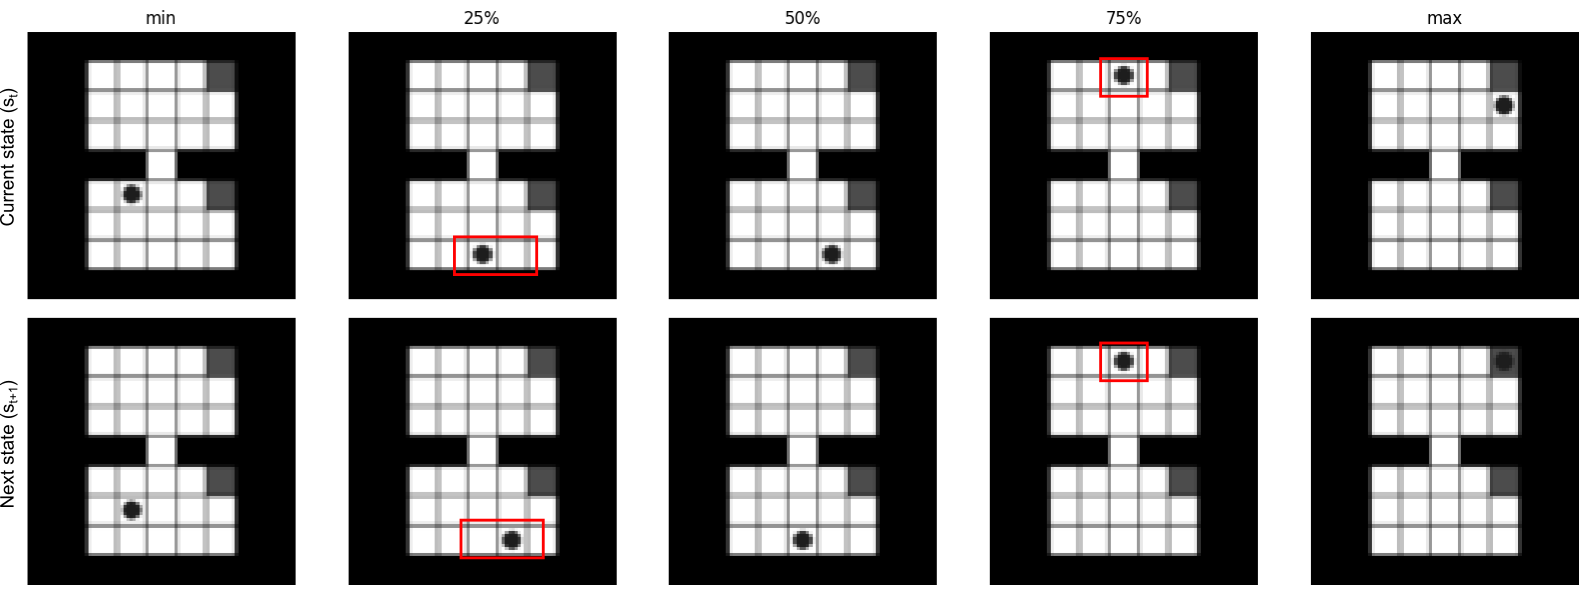
\includegraphics[width=\linewidth]{Results/grid_world/quartiles_images_per_50k.png}
%         \caption{DQN + PER}
%         \label{fig:quartiles_images_per_50k}
%     \end{subfigure}
%     \begin{subfigure}{1.\textwidth}
%         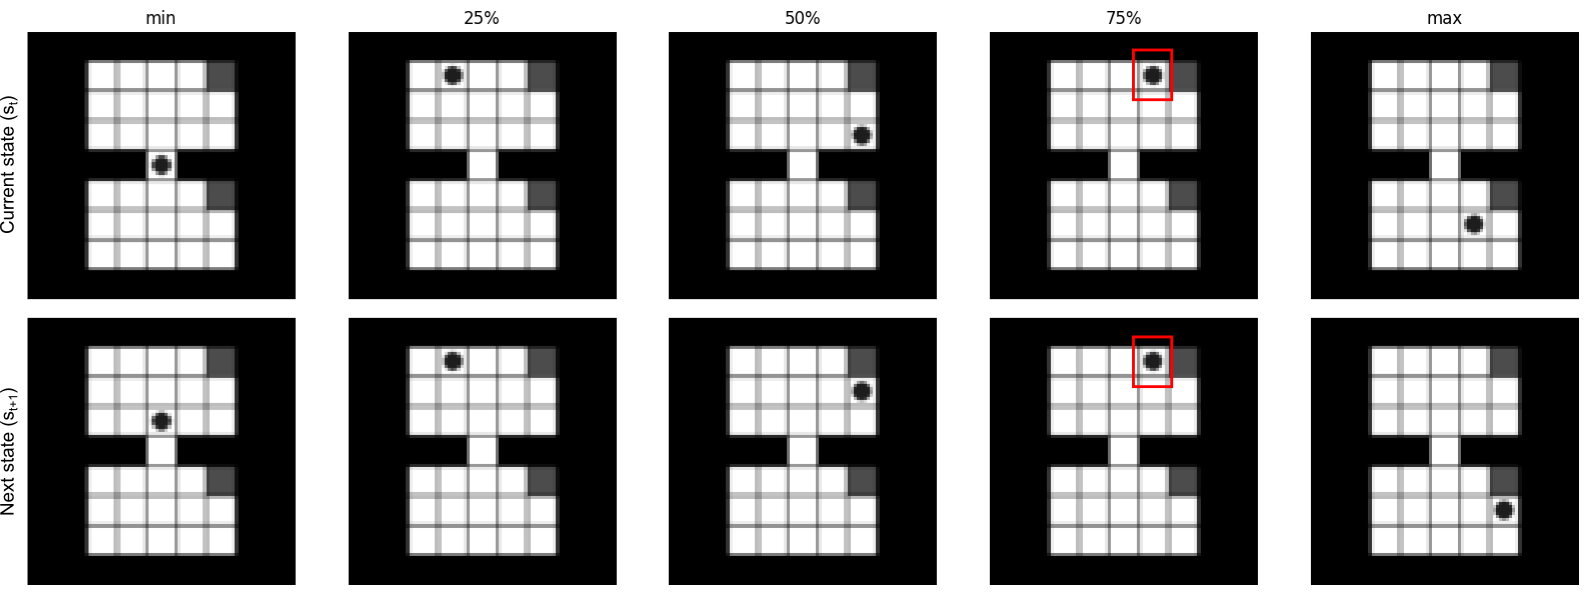
\includegraphics[width=\linewidth]{Results/grid_world/quartiles_images_dqn_mico_bpercn_50k.png}
%         \caption{DQN (MICO) + BPERcn}
%         \label{fig:quartiles_images_dqn_mico_bpercn_50k}
%     \end{subfigure}
%     \begin{subfigure}{1.\textwidth}
%         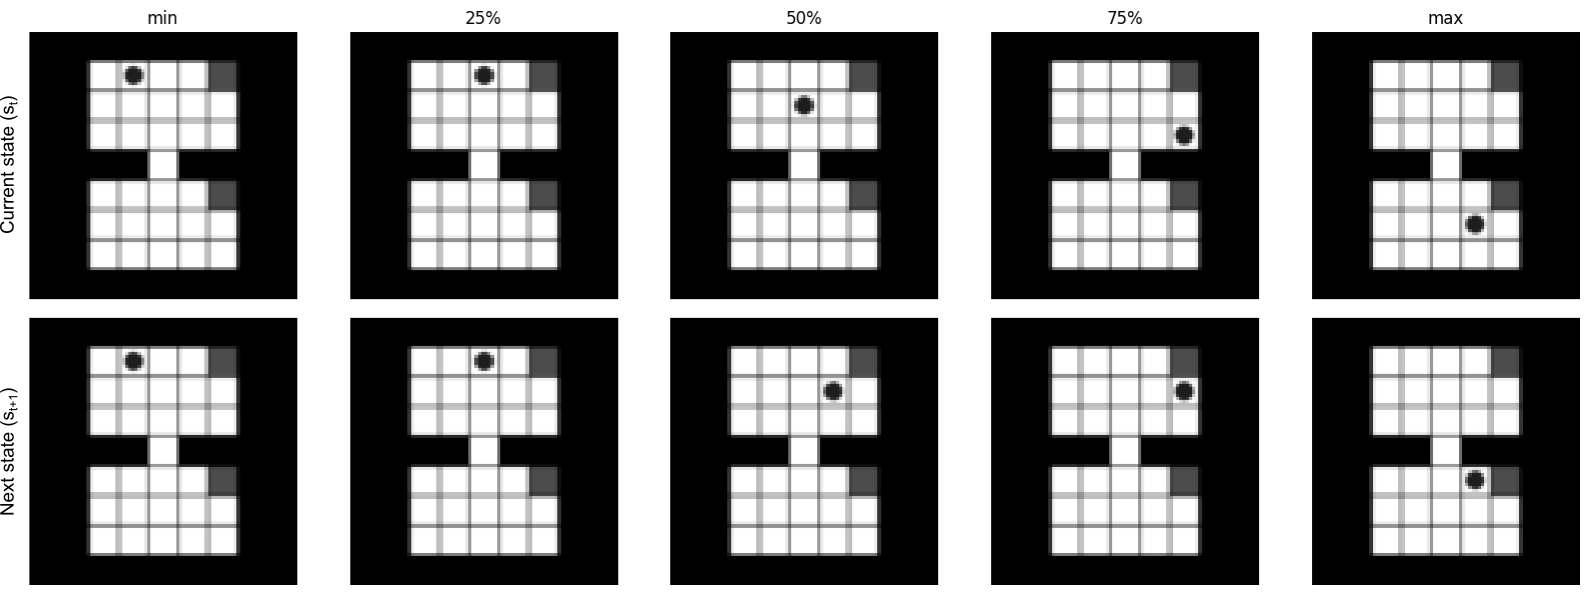
\includegraphics[width=\linewidth]{Results/grid_world/quartiles_images_dqn_mico_bperaa_50k.png}
%         \caption{DQN (MICO) + BPERaa}
%         \label{fig:quartiles_images_dqn_mico_bperaa_50k}
%     \end{subfigure}
%     \caption[Visual Inspection at the 50k time step]{\textbf{Visual Inspection at the 50k time step.} Frames corresponding to the main quartiles (min, 25\%, 50\%, 75\% and max) of priority values in the experience replay collected at the 50k time step, highlighting different problematic transitions with red colour. The top row shows the current states, and the bottom row shows the next states for each transition.}
%     \label{fig:quartiles_all_methods_50k}
% \end{figure}

% \section{Priority Weight Sweep Results}
% \label{append:priority_weight_sweep}

% \begin{figure}[H]
%     \centering
%     \begin{subfigure}{0.45\textwidth}
%     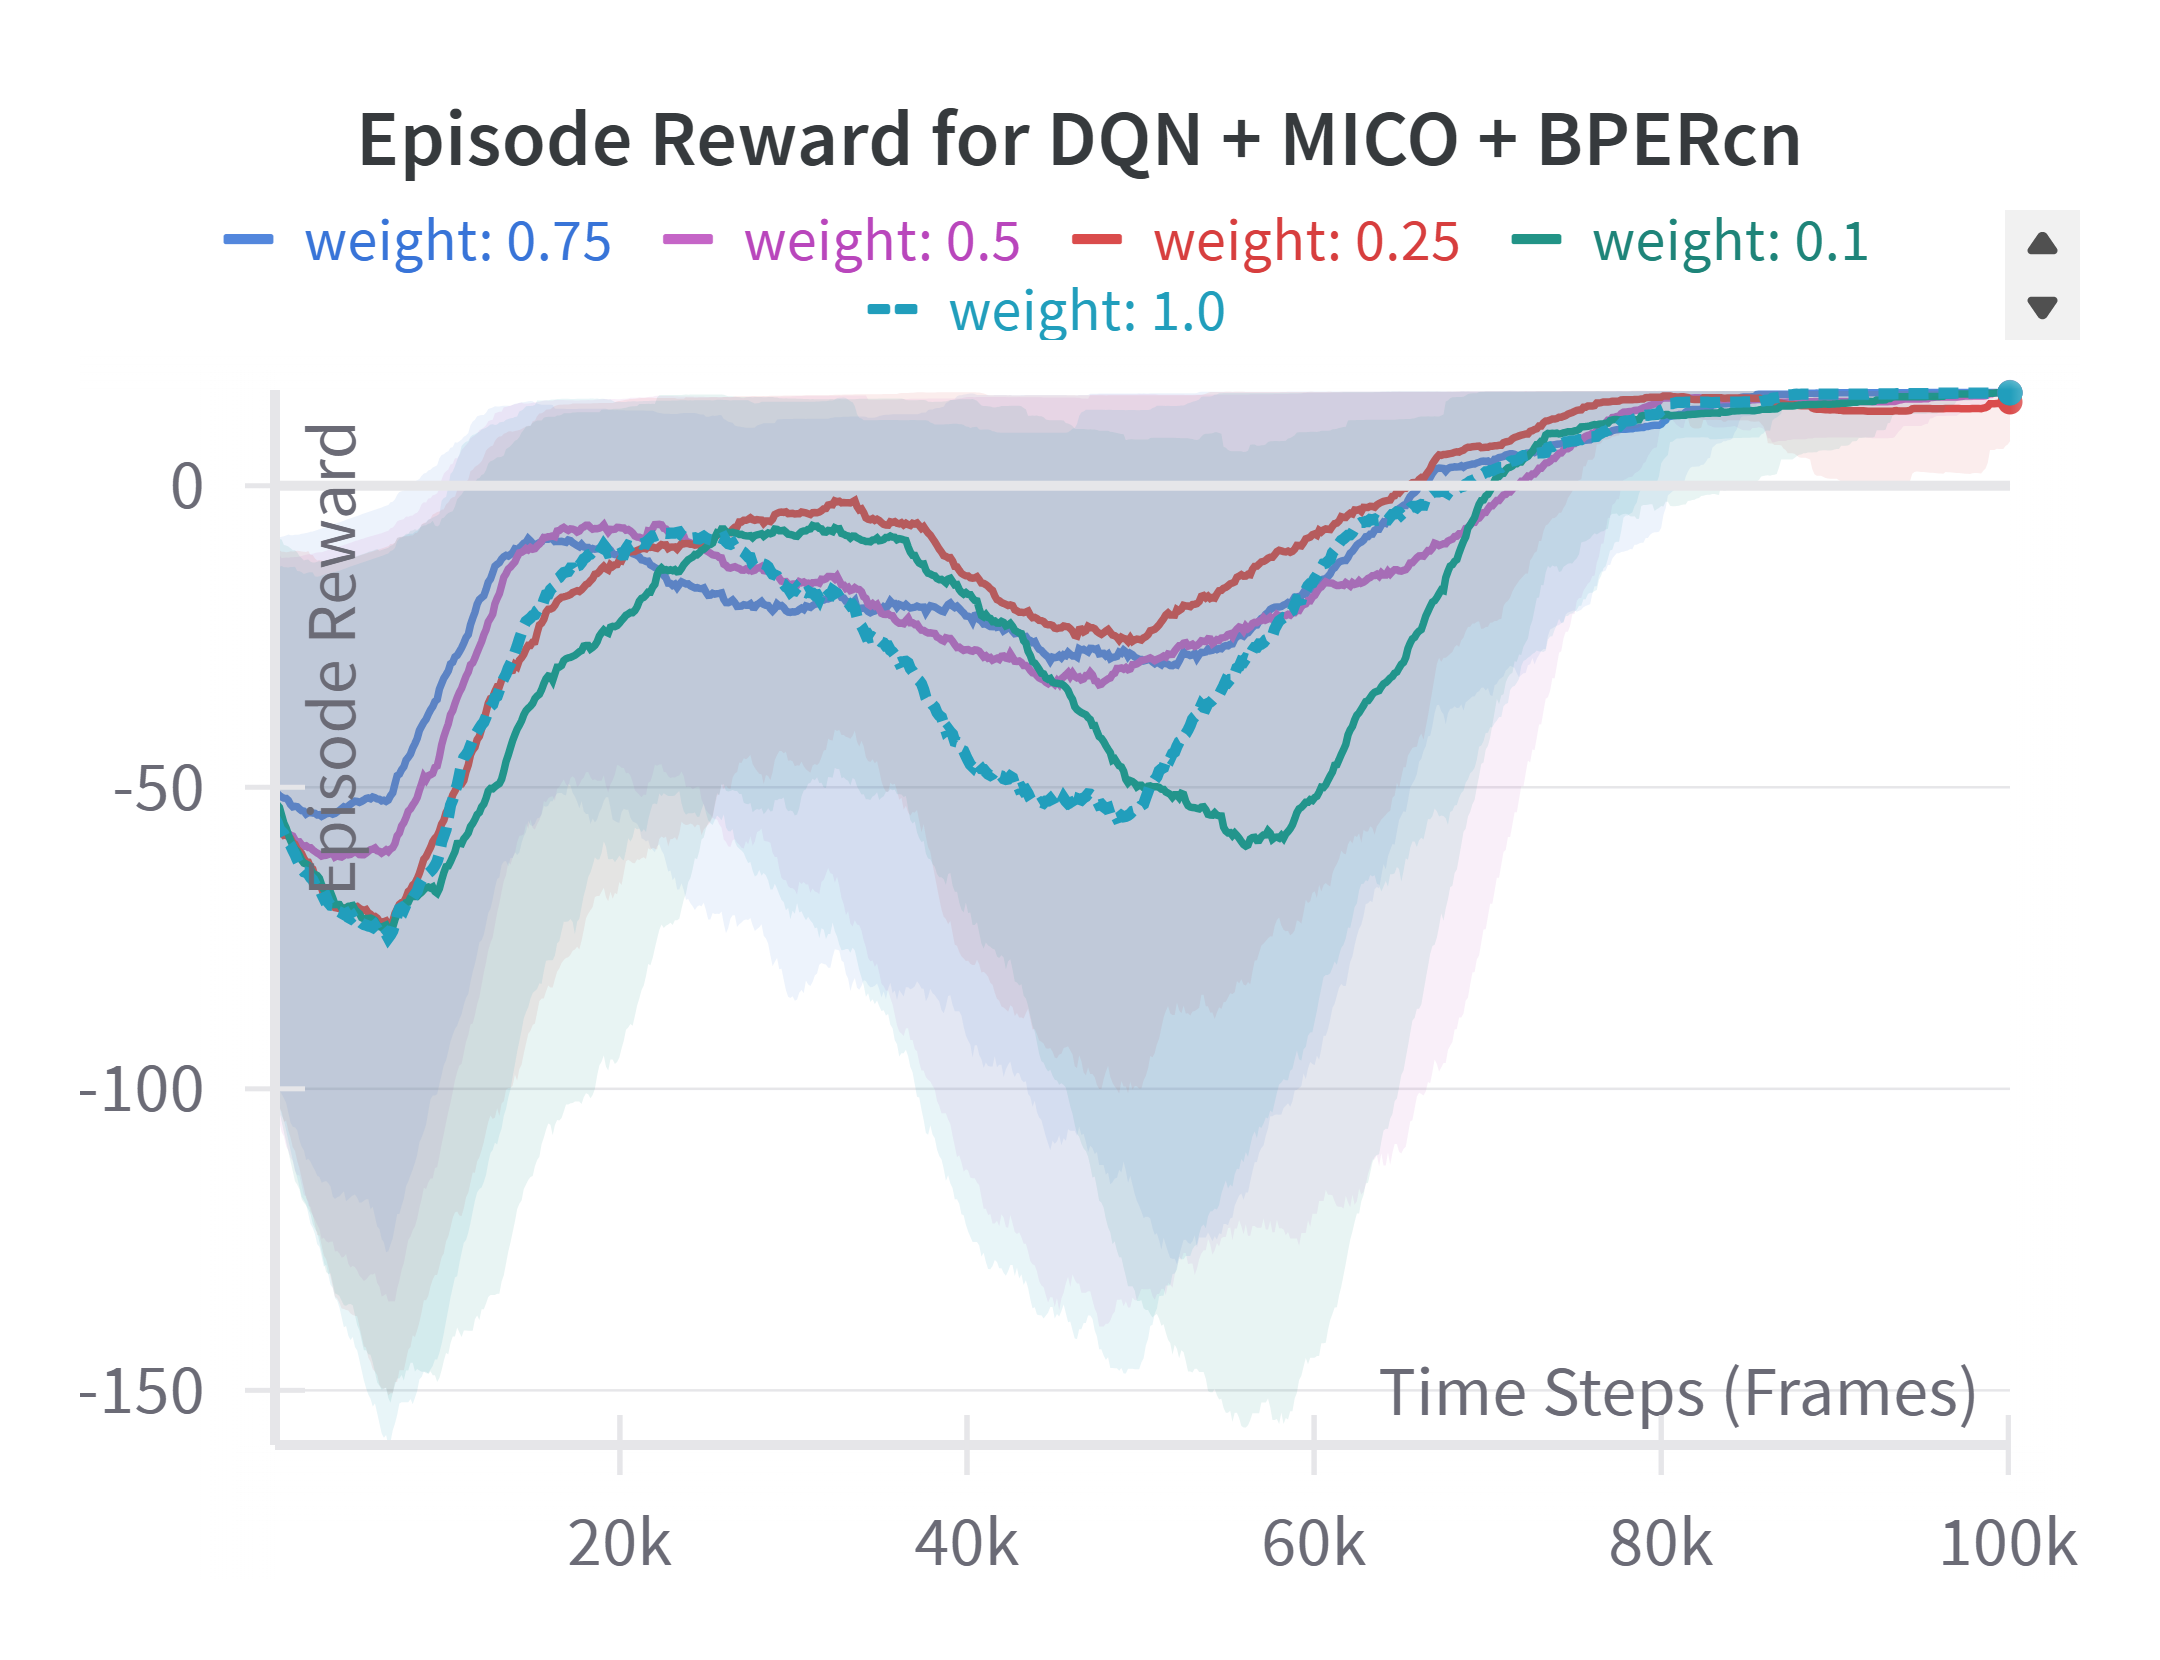
\includegraphics[width=\linewidth]{Results/grid_world/sweep_bpercn_grid_world.png}
%         \caption{Sweep BPERcn}
%         \label{fig:sweep_bpercn_grid_world}
%     \end{subfigure}
%     \hfill
%     \begin{subfigure}{0.45\textwidth}
%         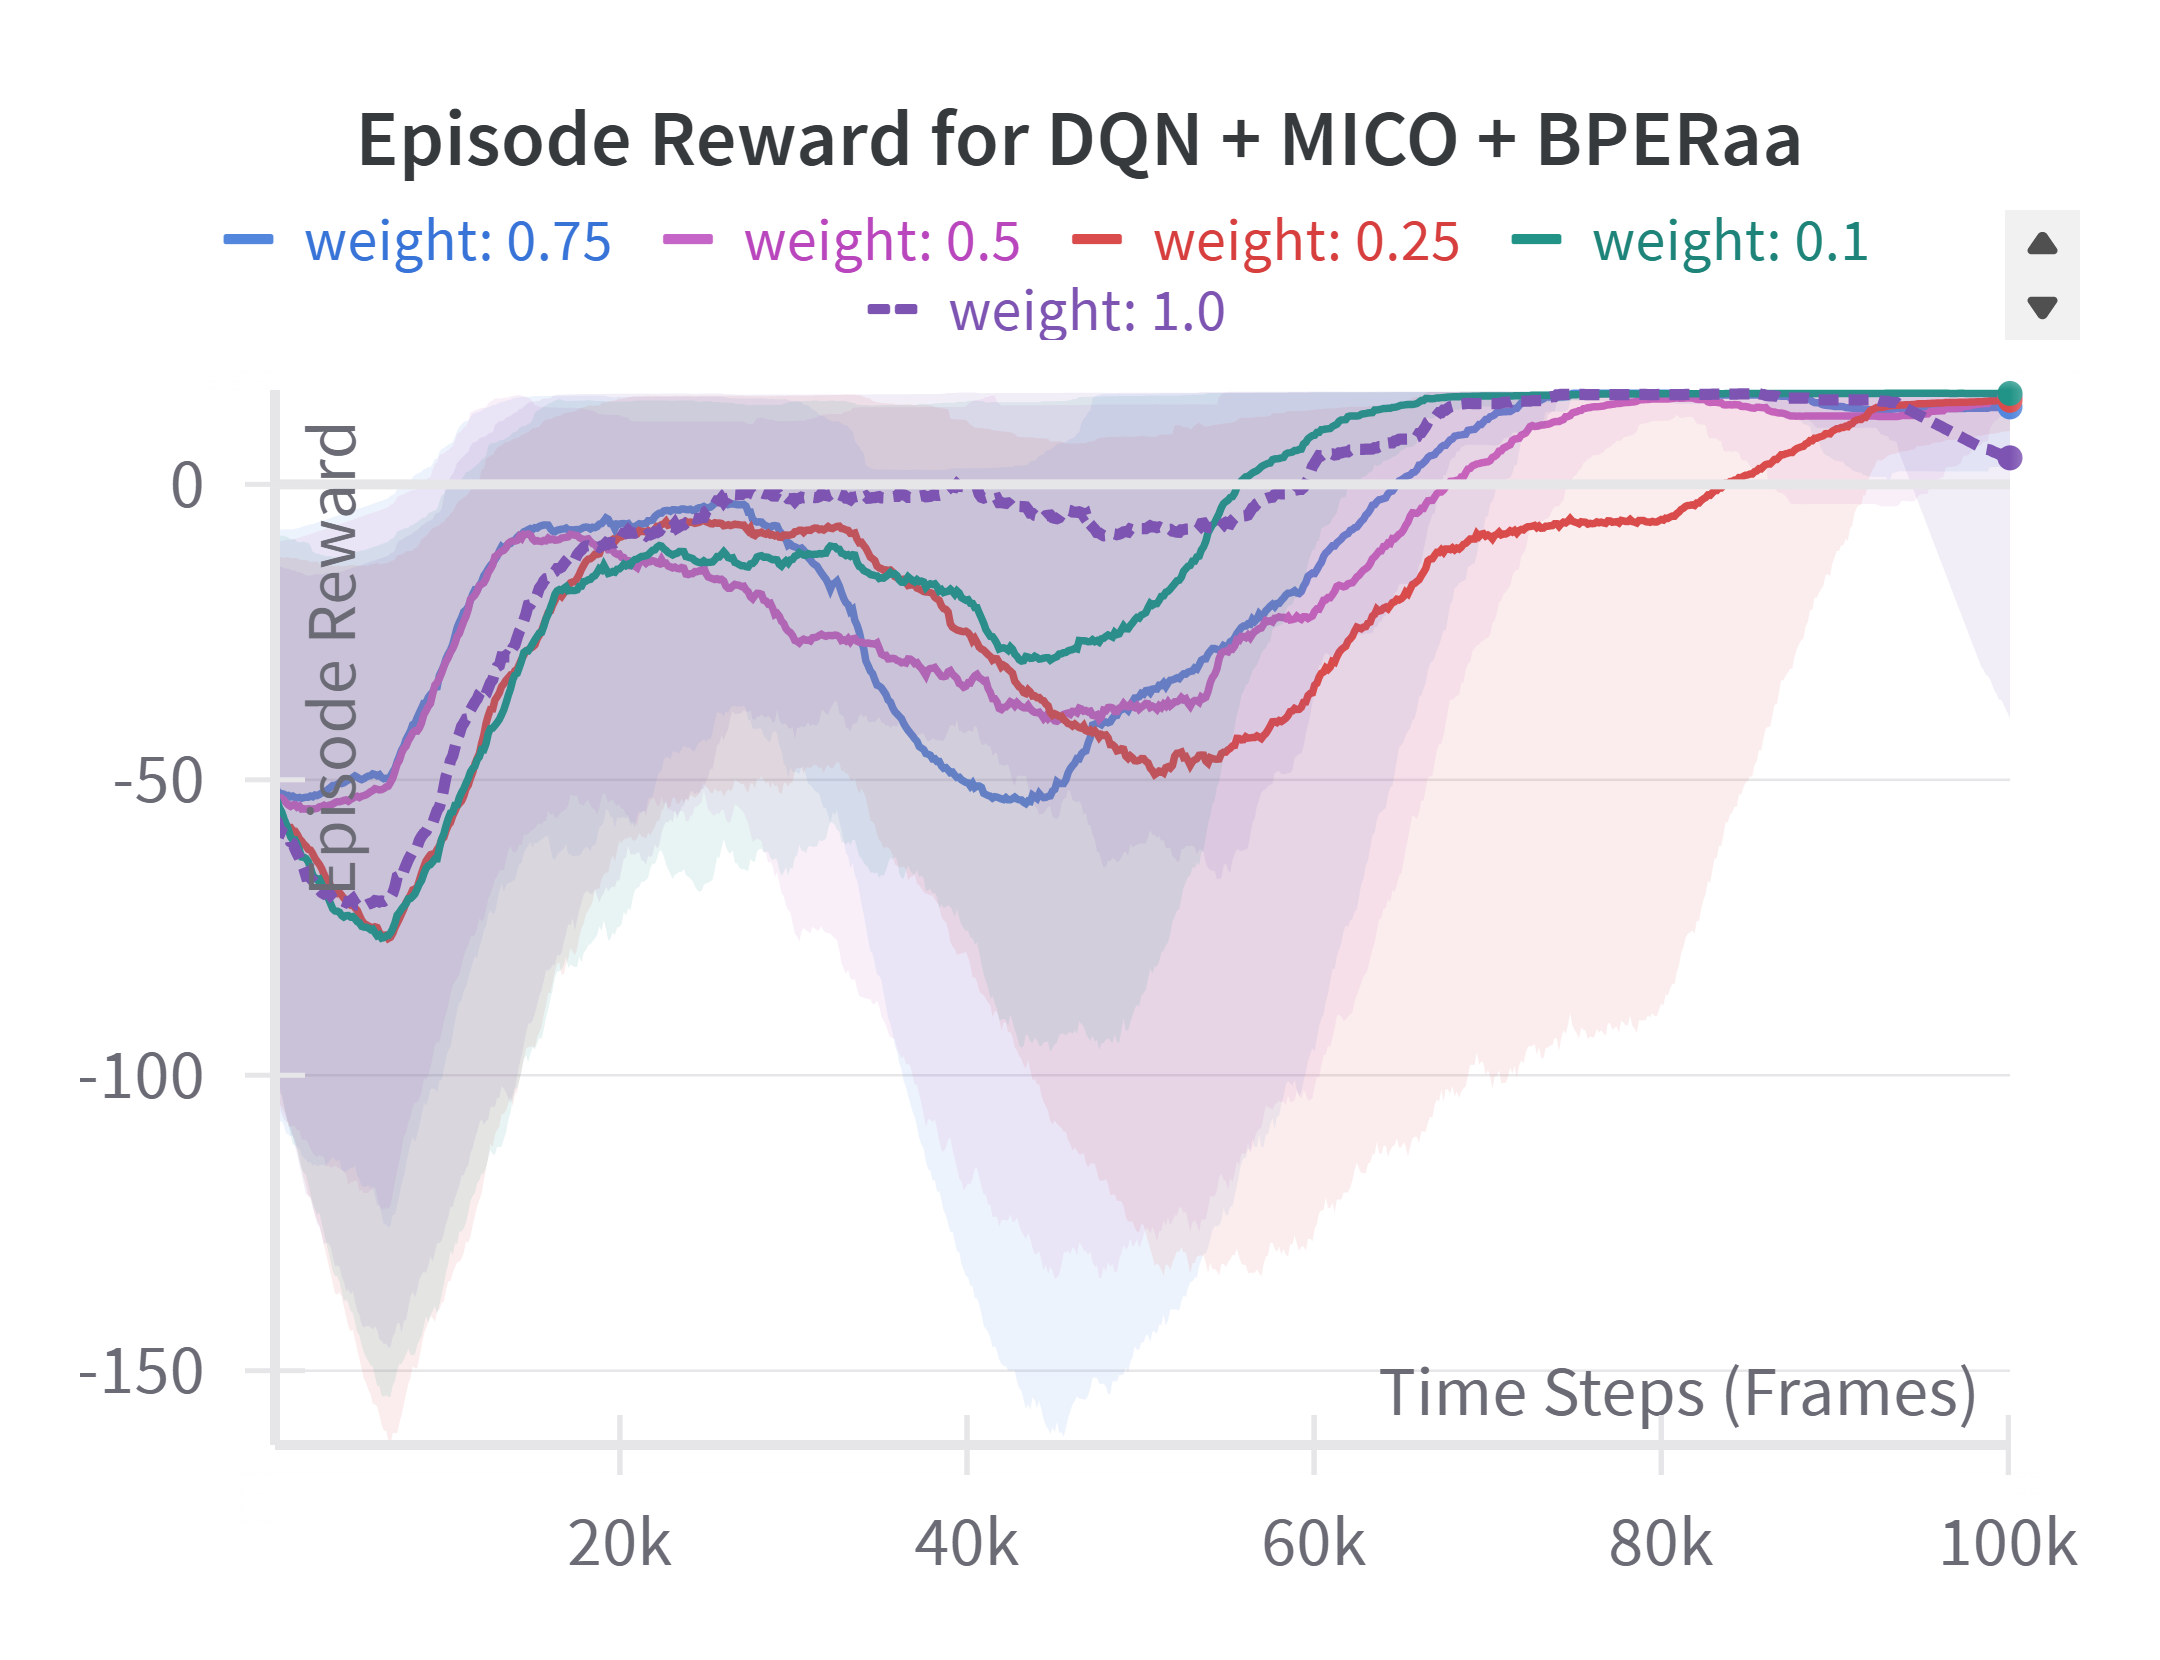
\includegraphics[width=\linewidth]{Results/grid_world/sweep_bperaa_grid_world.png}
%         \caption{Sweep BPERcn}
%         \label{fig:sweep_bperaa_grid_world}
%     \end{subfigure}
%     \caption[Priority Weight Sweep in Grid World]{\textbf{Priority Weight Sweep in Grid World.} Episode reward sweep over priority weights with values 0.1, 0.25, 0.5, 0.75, and 1.0, averaged with a moving window of 100 episodes across 5 independent executions over time. Shaded regions represent the variability for each method. The values are calculated for (a) the current-next strategy (BPERcn) and (b) the all-vs-all strategy (BPERaa).}
%     \label{fig:sweep_methods_grid_world}
% \end{figure}

% \section{Mountain Car and CartPole with Priority Weight 1.0}
% \label{append:results_priority_weight_1_0}
% \begin{figure}[H]
%     \centering
%     \begin{subfigure}{0.45\textwidth}
%     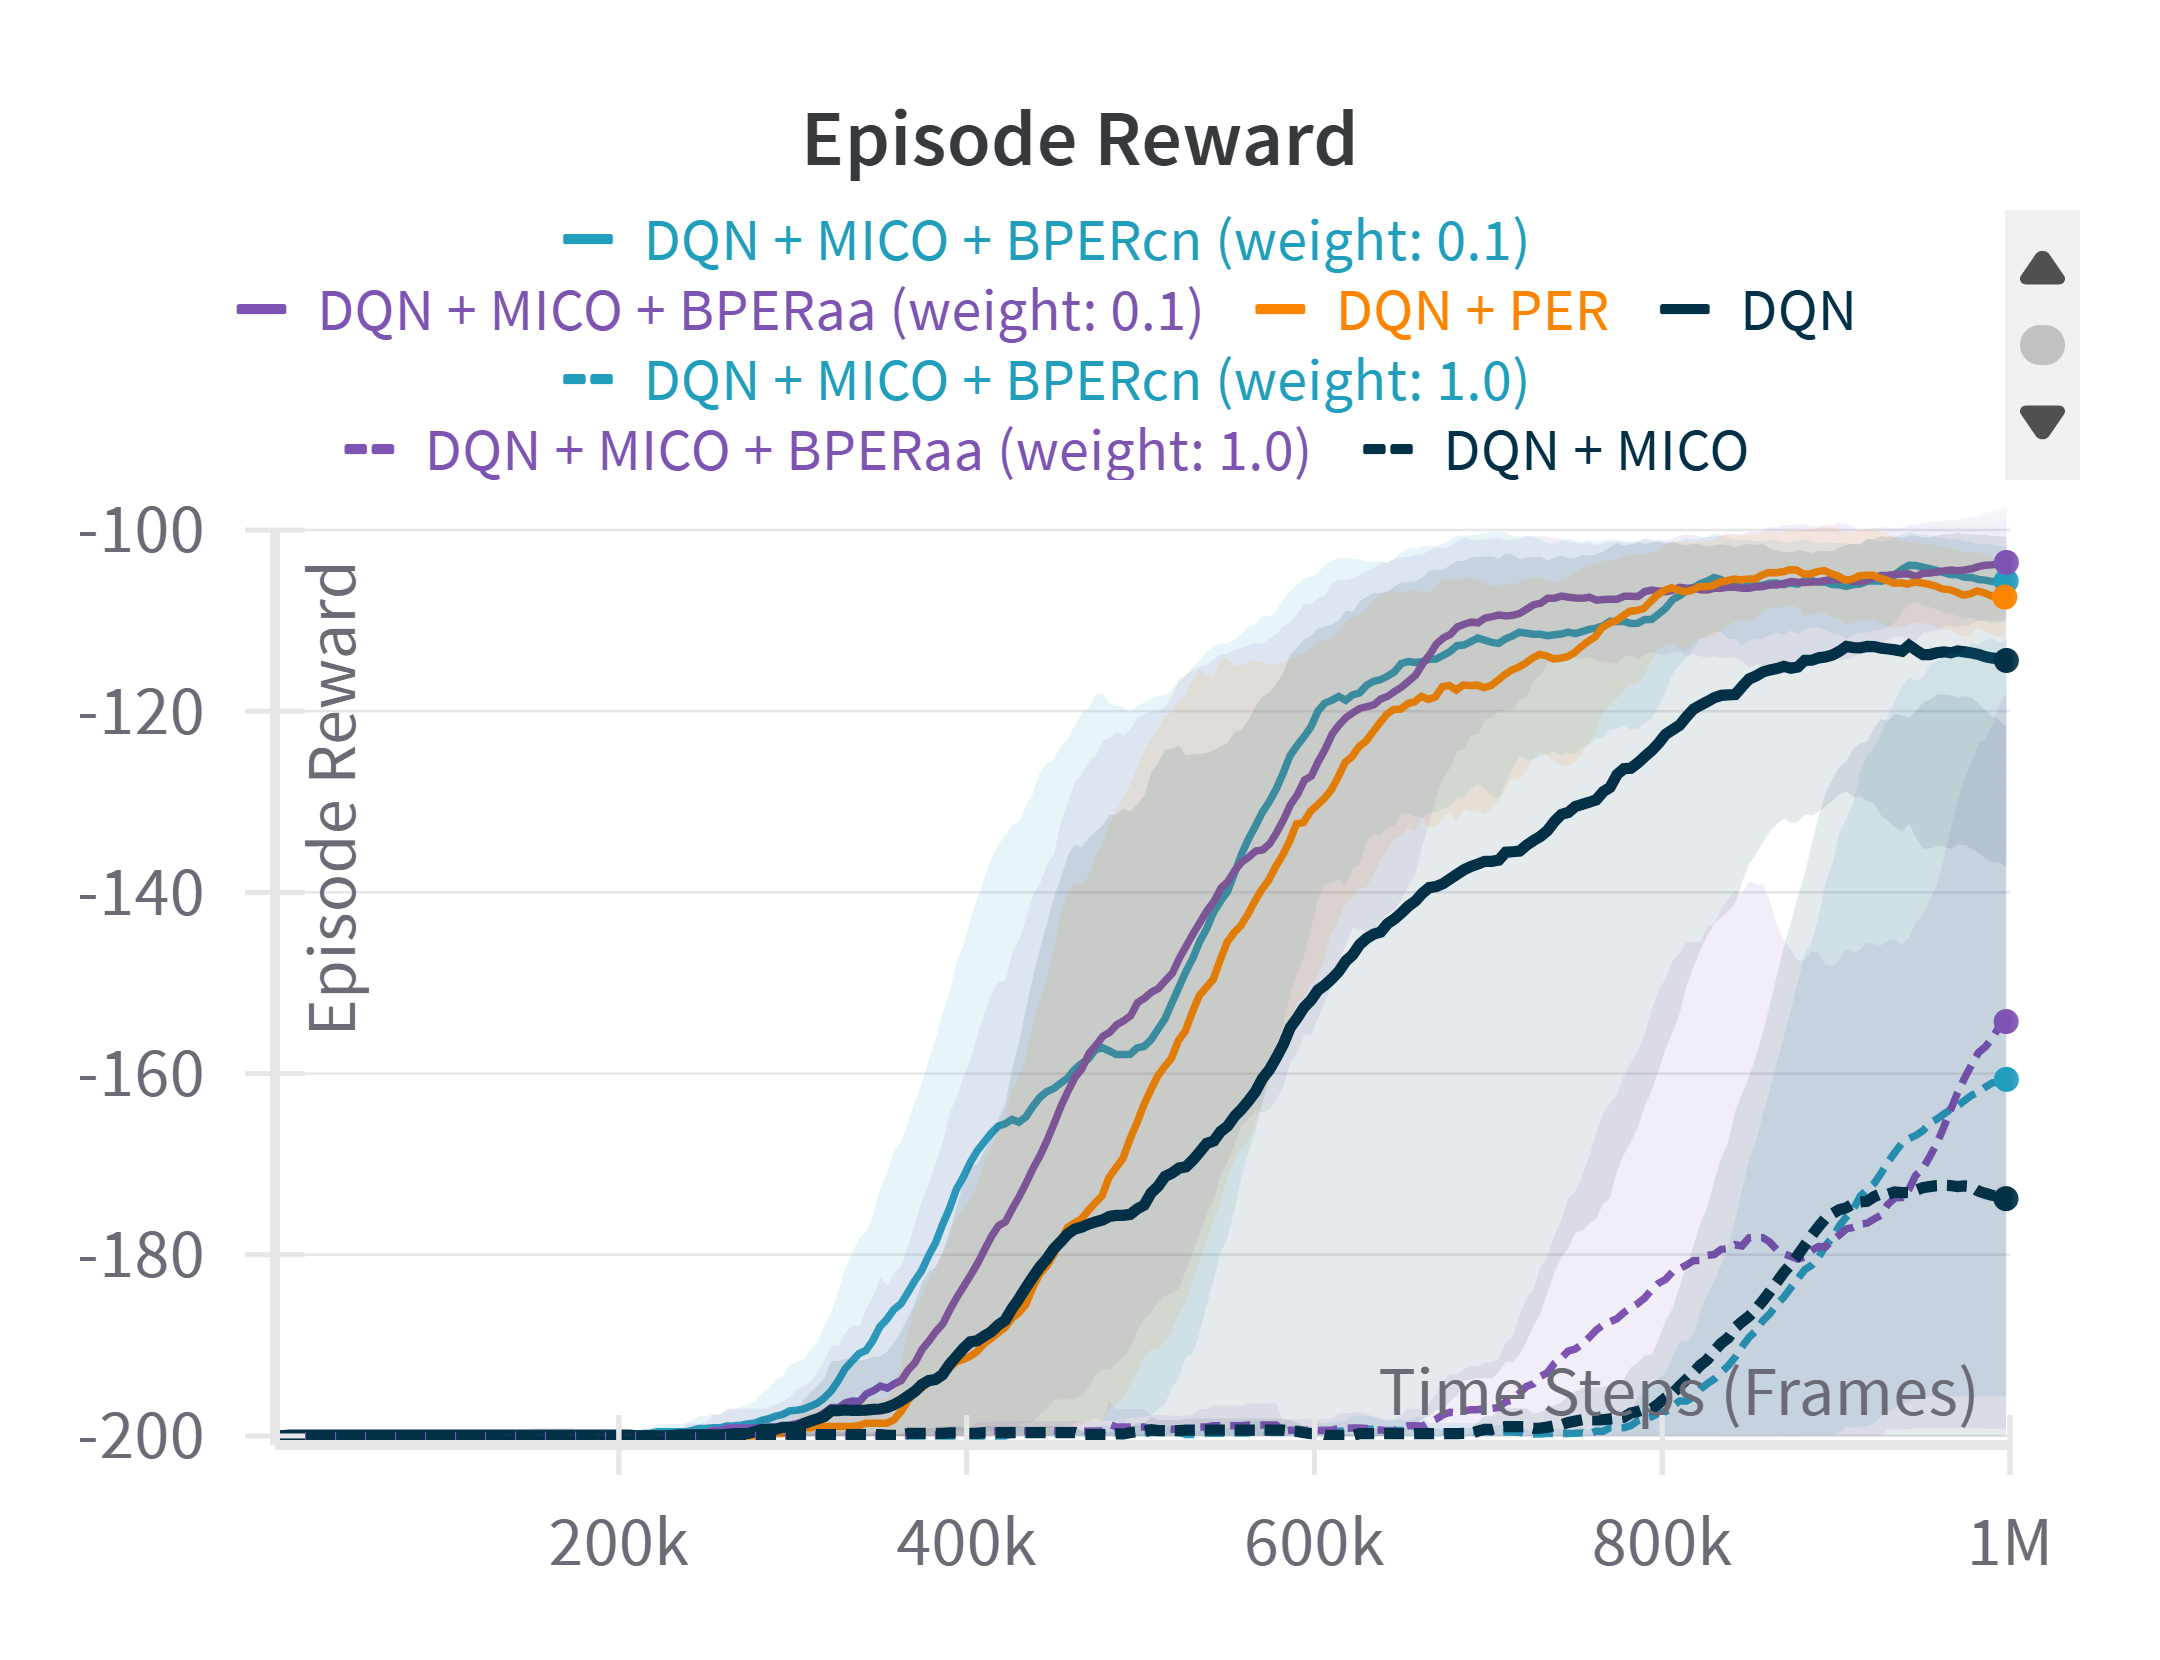
\includegraphics[width=\linewidth]{Results/general_results/return_mountain_car_weigh_1.png}
%         \caption{Mountain Car}
%         \label{fig:return_mountain_car_weigh_1}
%     \end{subfigure}
%     \hfill
%     \begin{subfigure}{0.45\textwidth}
%         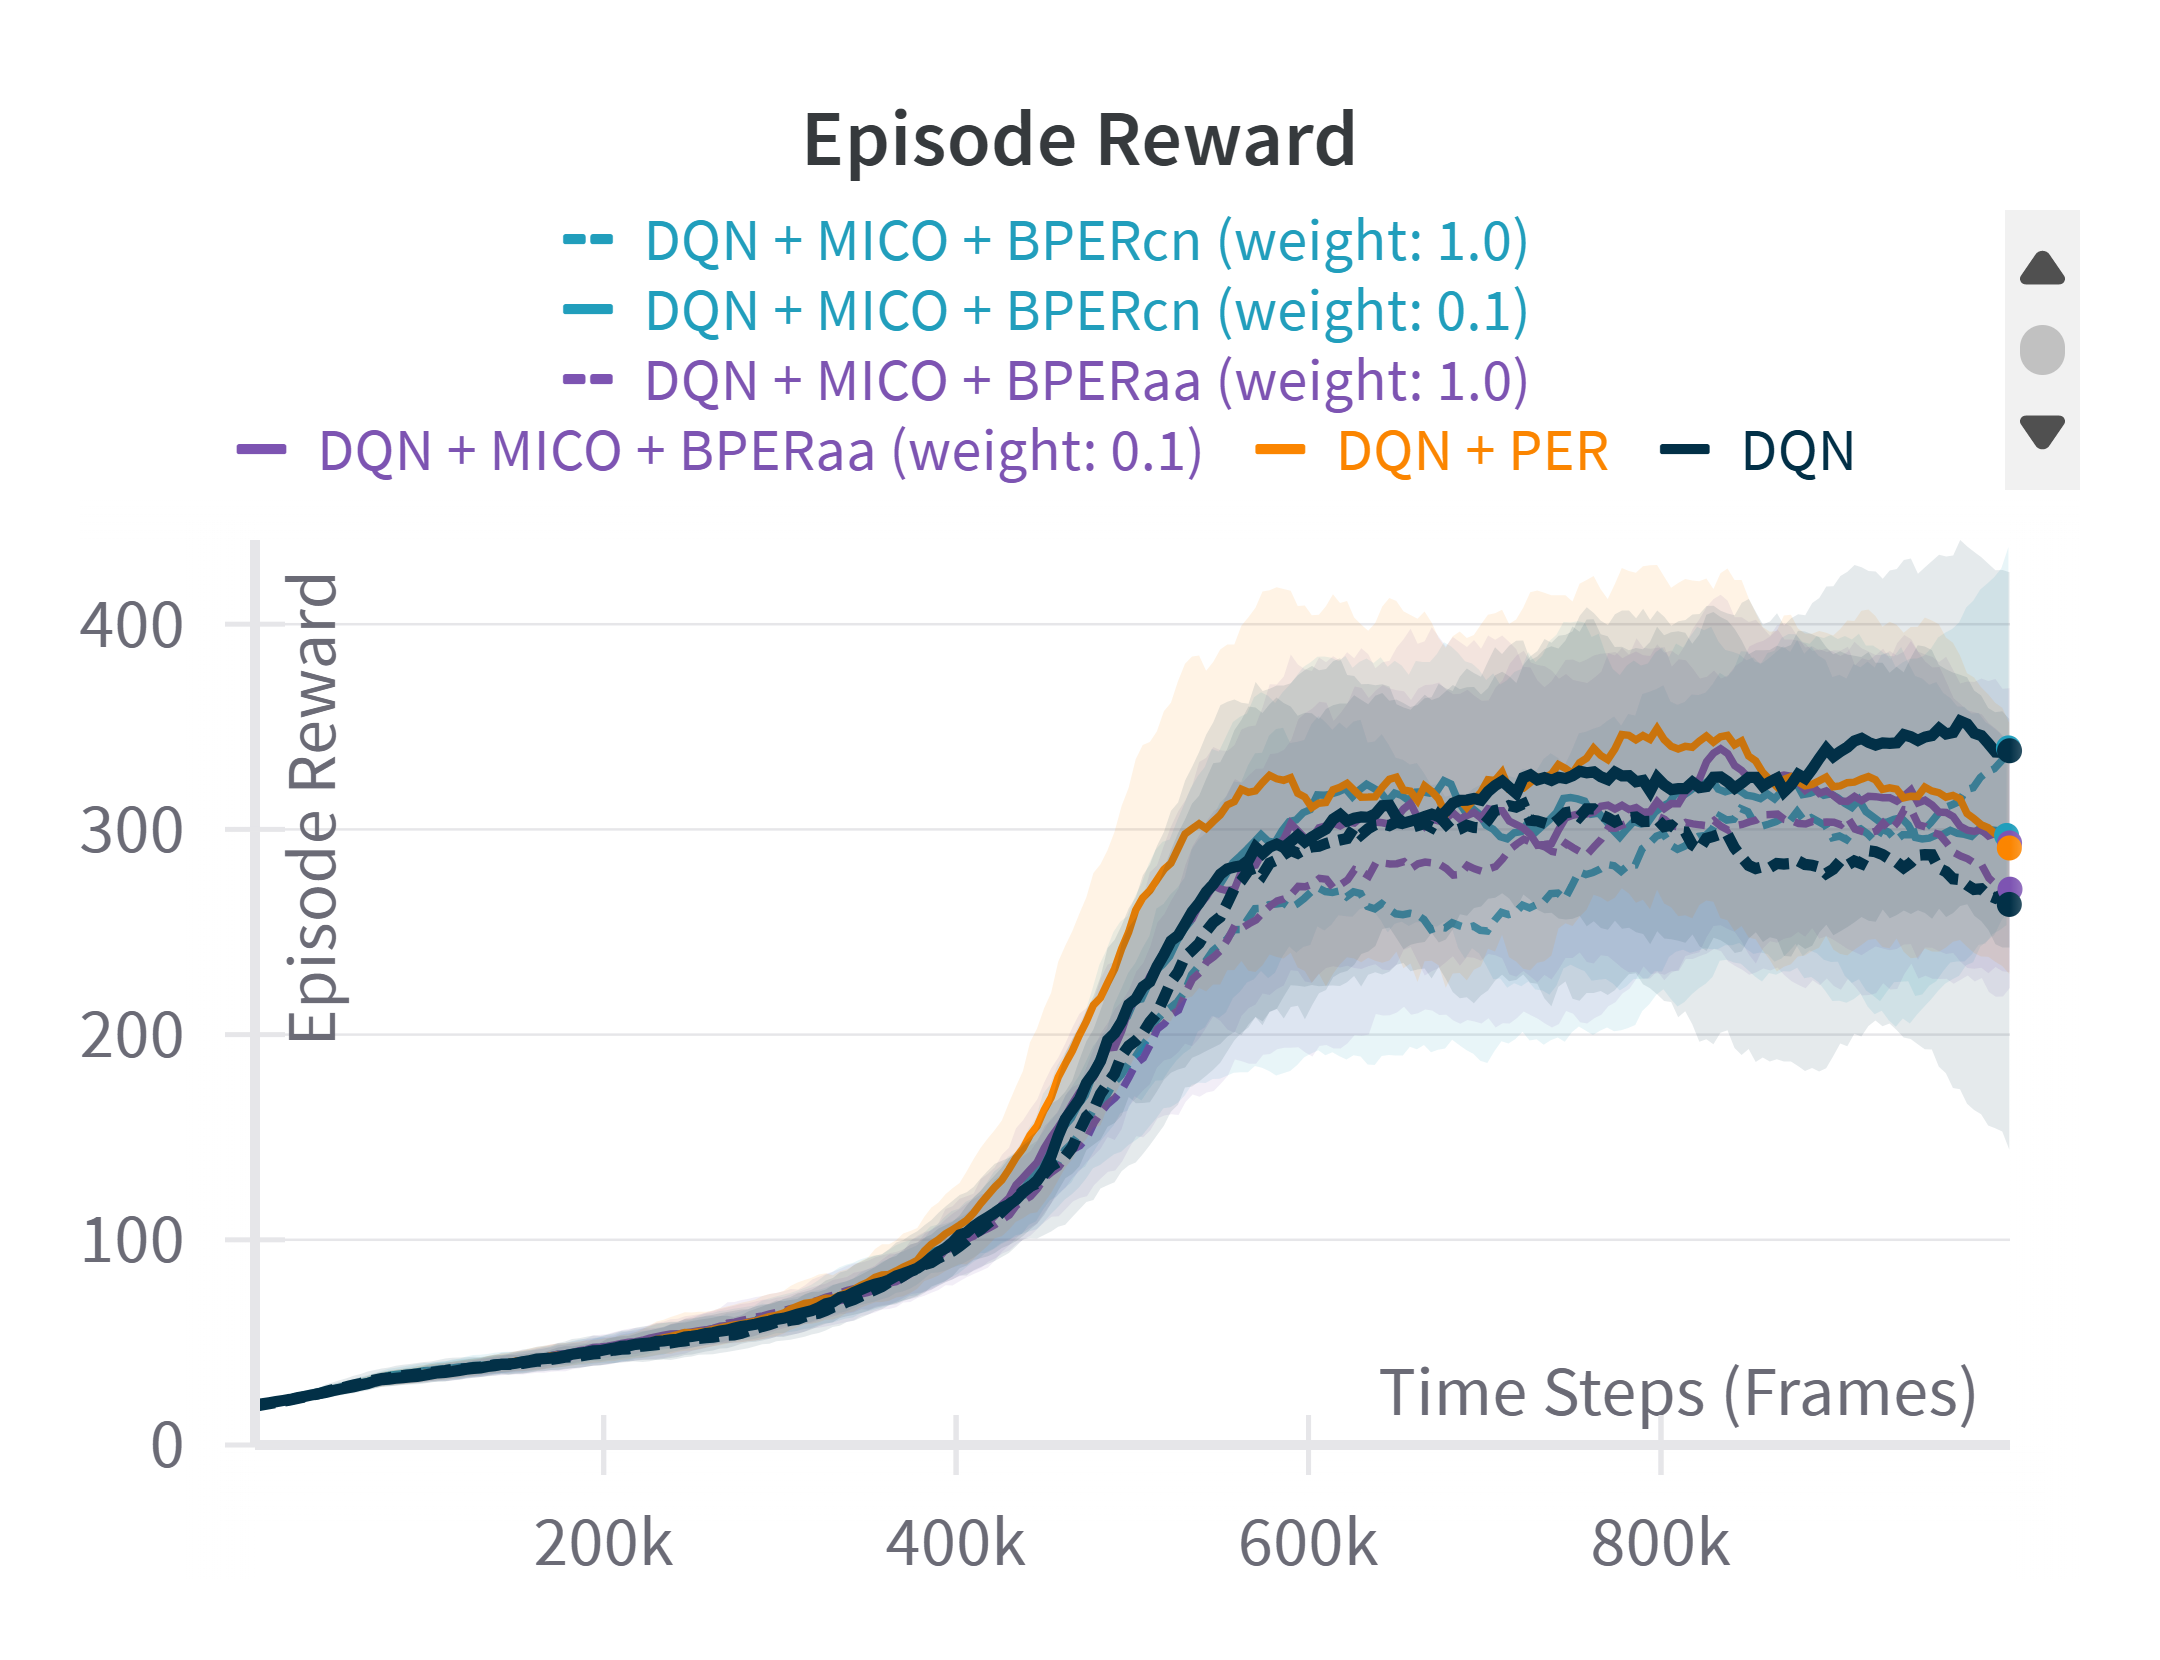
\includegraphics[width=\linewidth]{Results/general_results/return_cartpolev1_weight_1.png}
%         \caption{CartPole}
%         \label{fig:return_cartpolev1_weight_1}
%     \end{subfigure}
%     \caption[Episode Reward in Classical Environments using Priority Weight 1.0]{\textbf{Episode Reward in Classical Environments using Priority Weight 1.0} Episode reward performance over time, averaged with a moving window of 100 episodes across 5 independent executions, with shaded regions representing the variability for each method. The values are calculated in four different environments: (a) MountainCar-v0, (b) LunarLander-v1, (c) CartPole-v1, and (d) Acrobot-v1.}
%     \label{fig:return_methods_weight_1}
% \end{figure}

% \section{Validation Episode Reward}
% \label{append:validation_results}

% \begin{figure}[H]
%     \centering
%     \begin{subfigure}{0.45\textwidth}
%     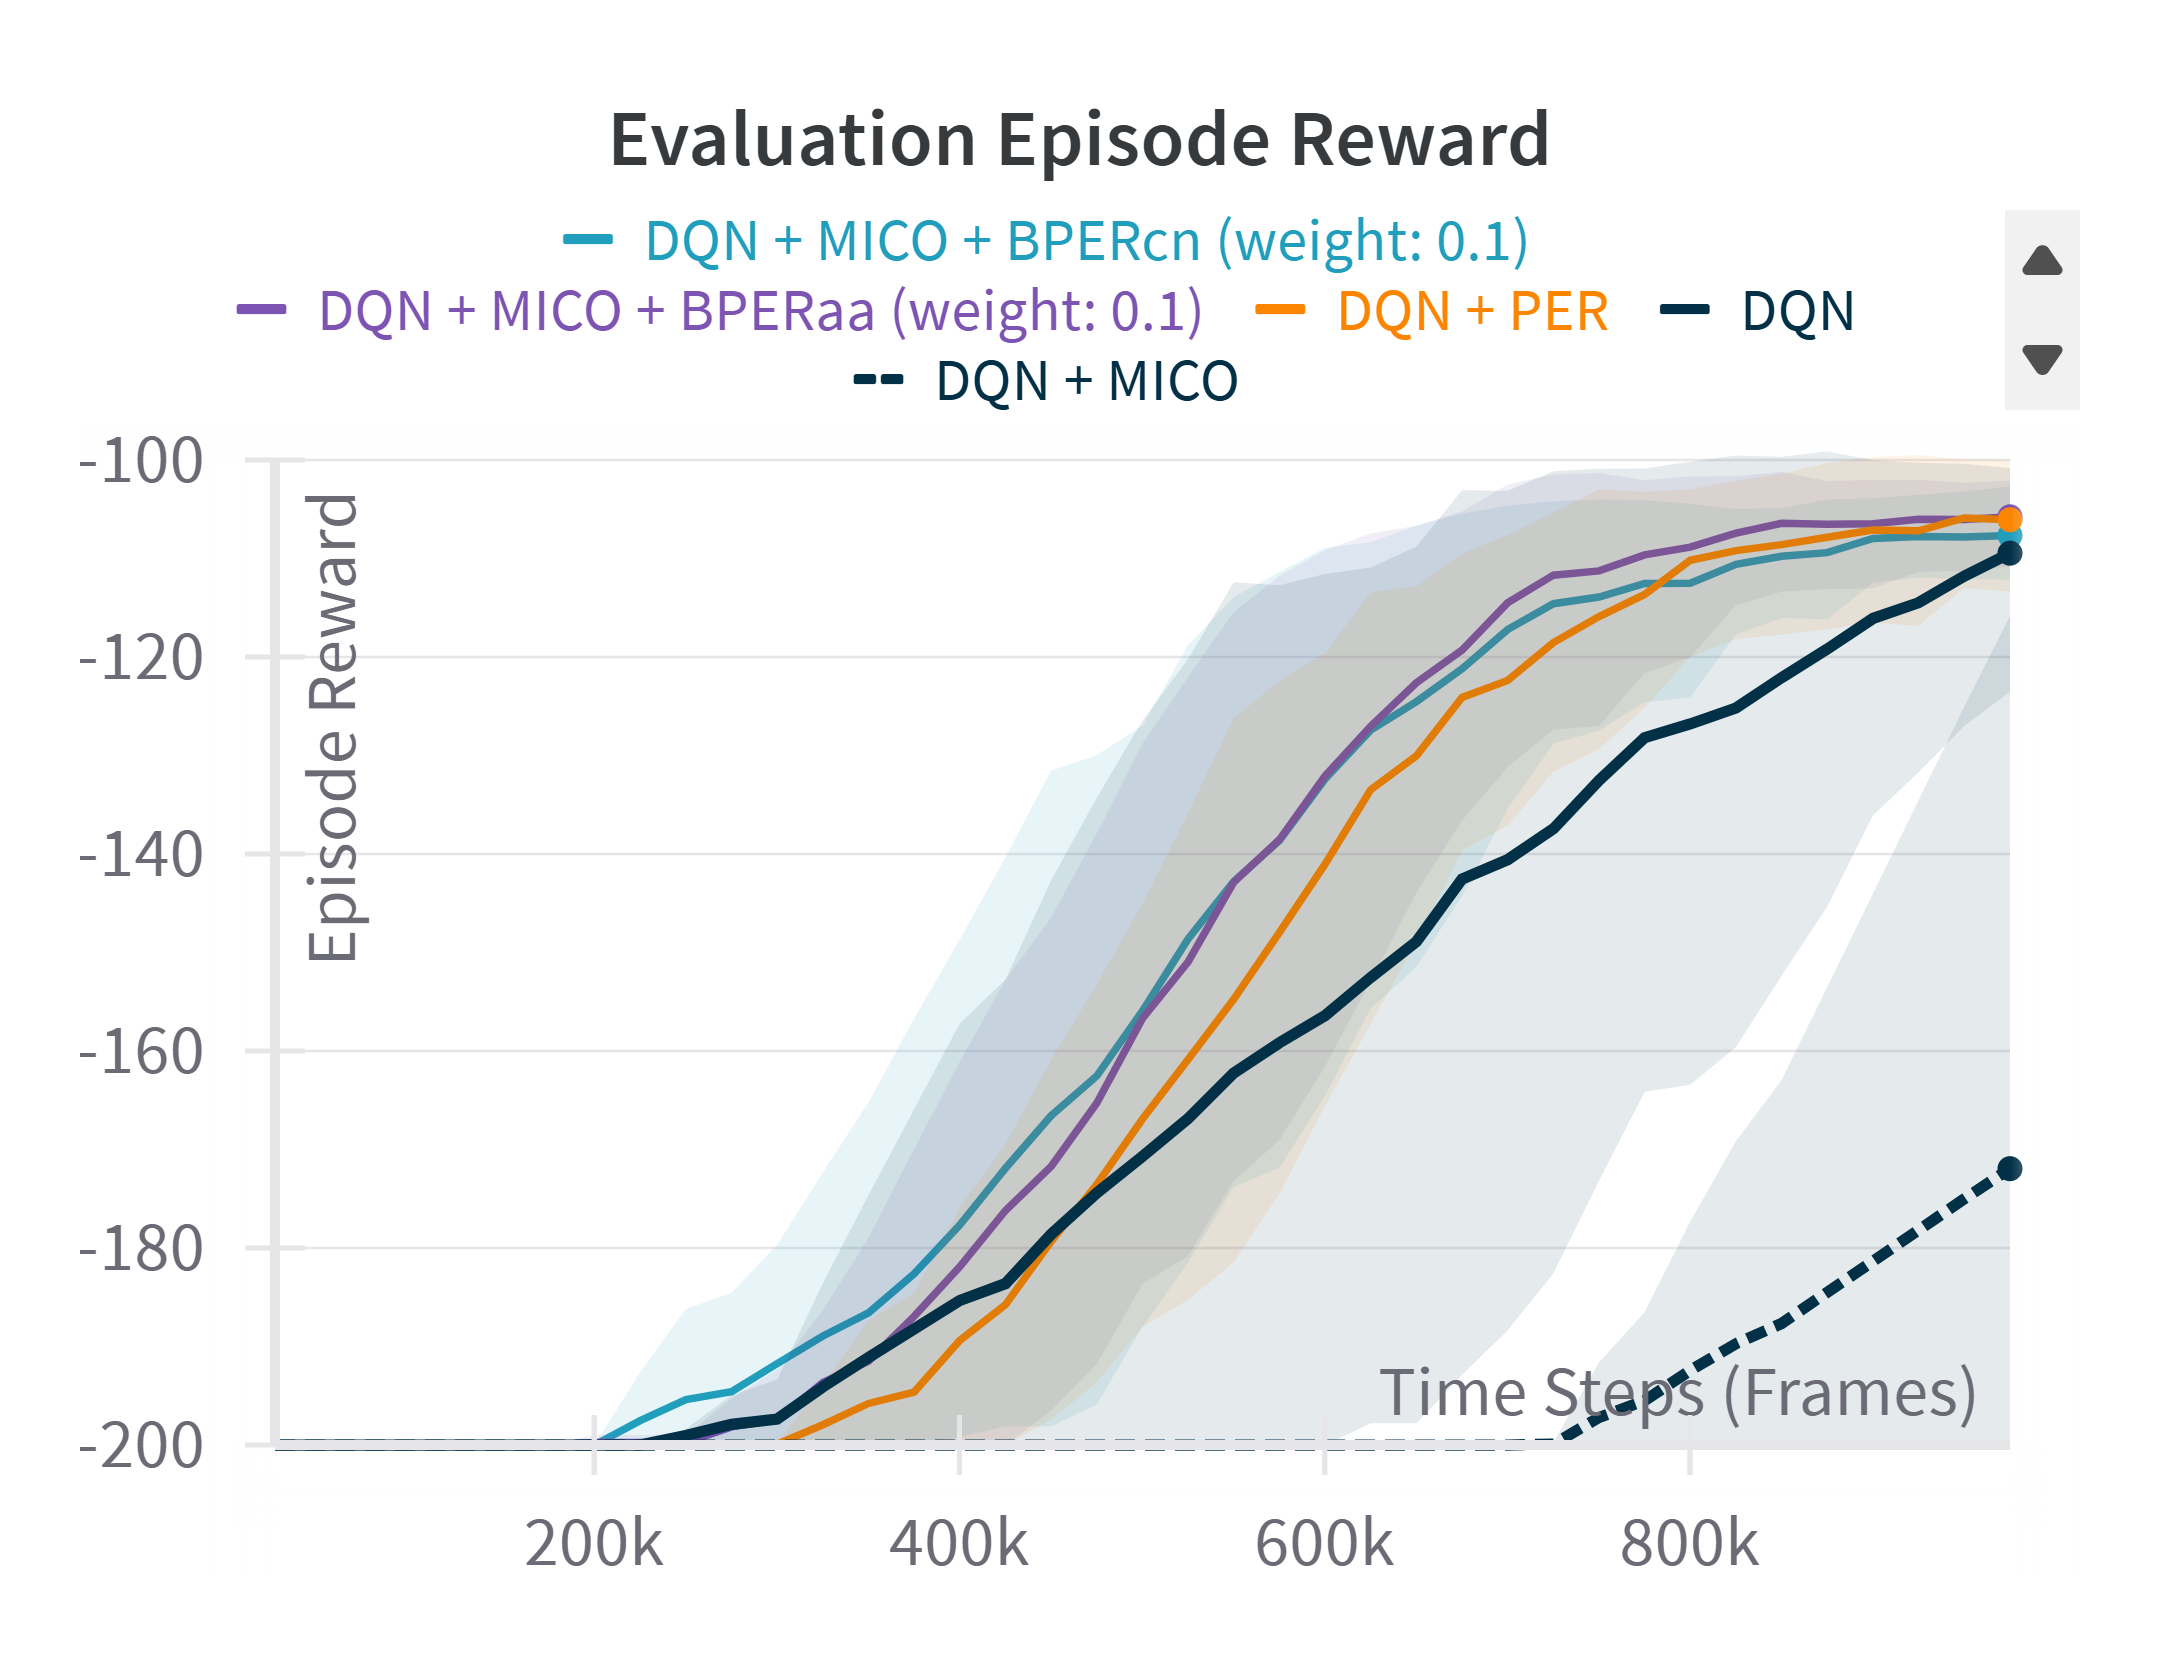
\includegraphics[width=\linewidth]{Results/general_results/eval_return_mountain_car.png}
%         \caption{MountainCar-v0}
%         \label{fig:eval_return_mountain_car}
%     \end{subfigure}
%     \hfill
%     \begin{subfigure}{0.45\textwidth}
%         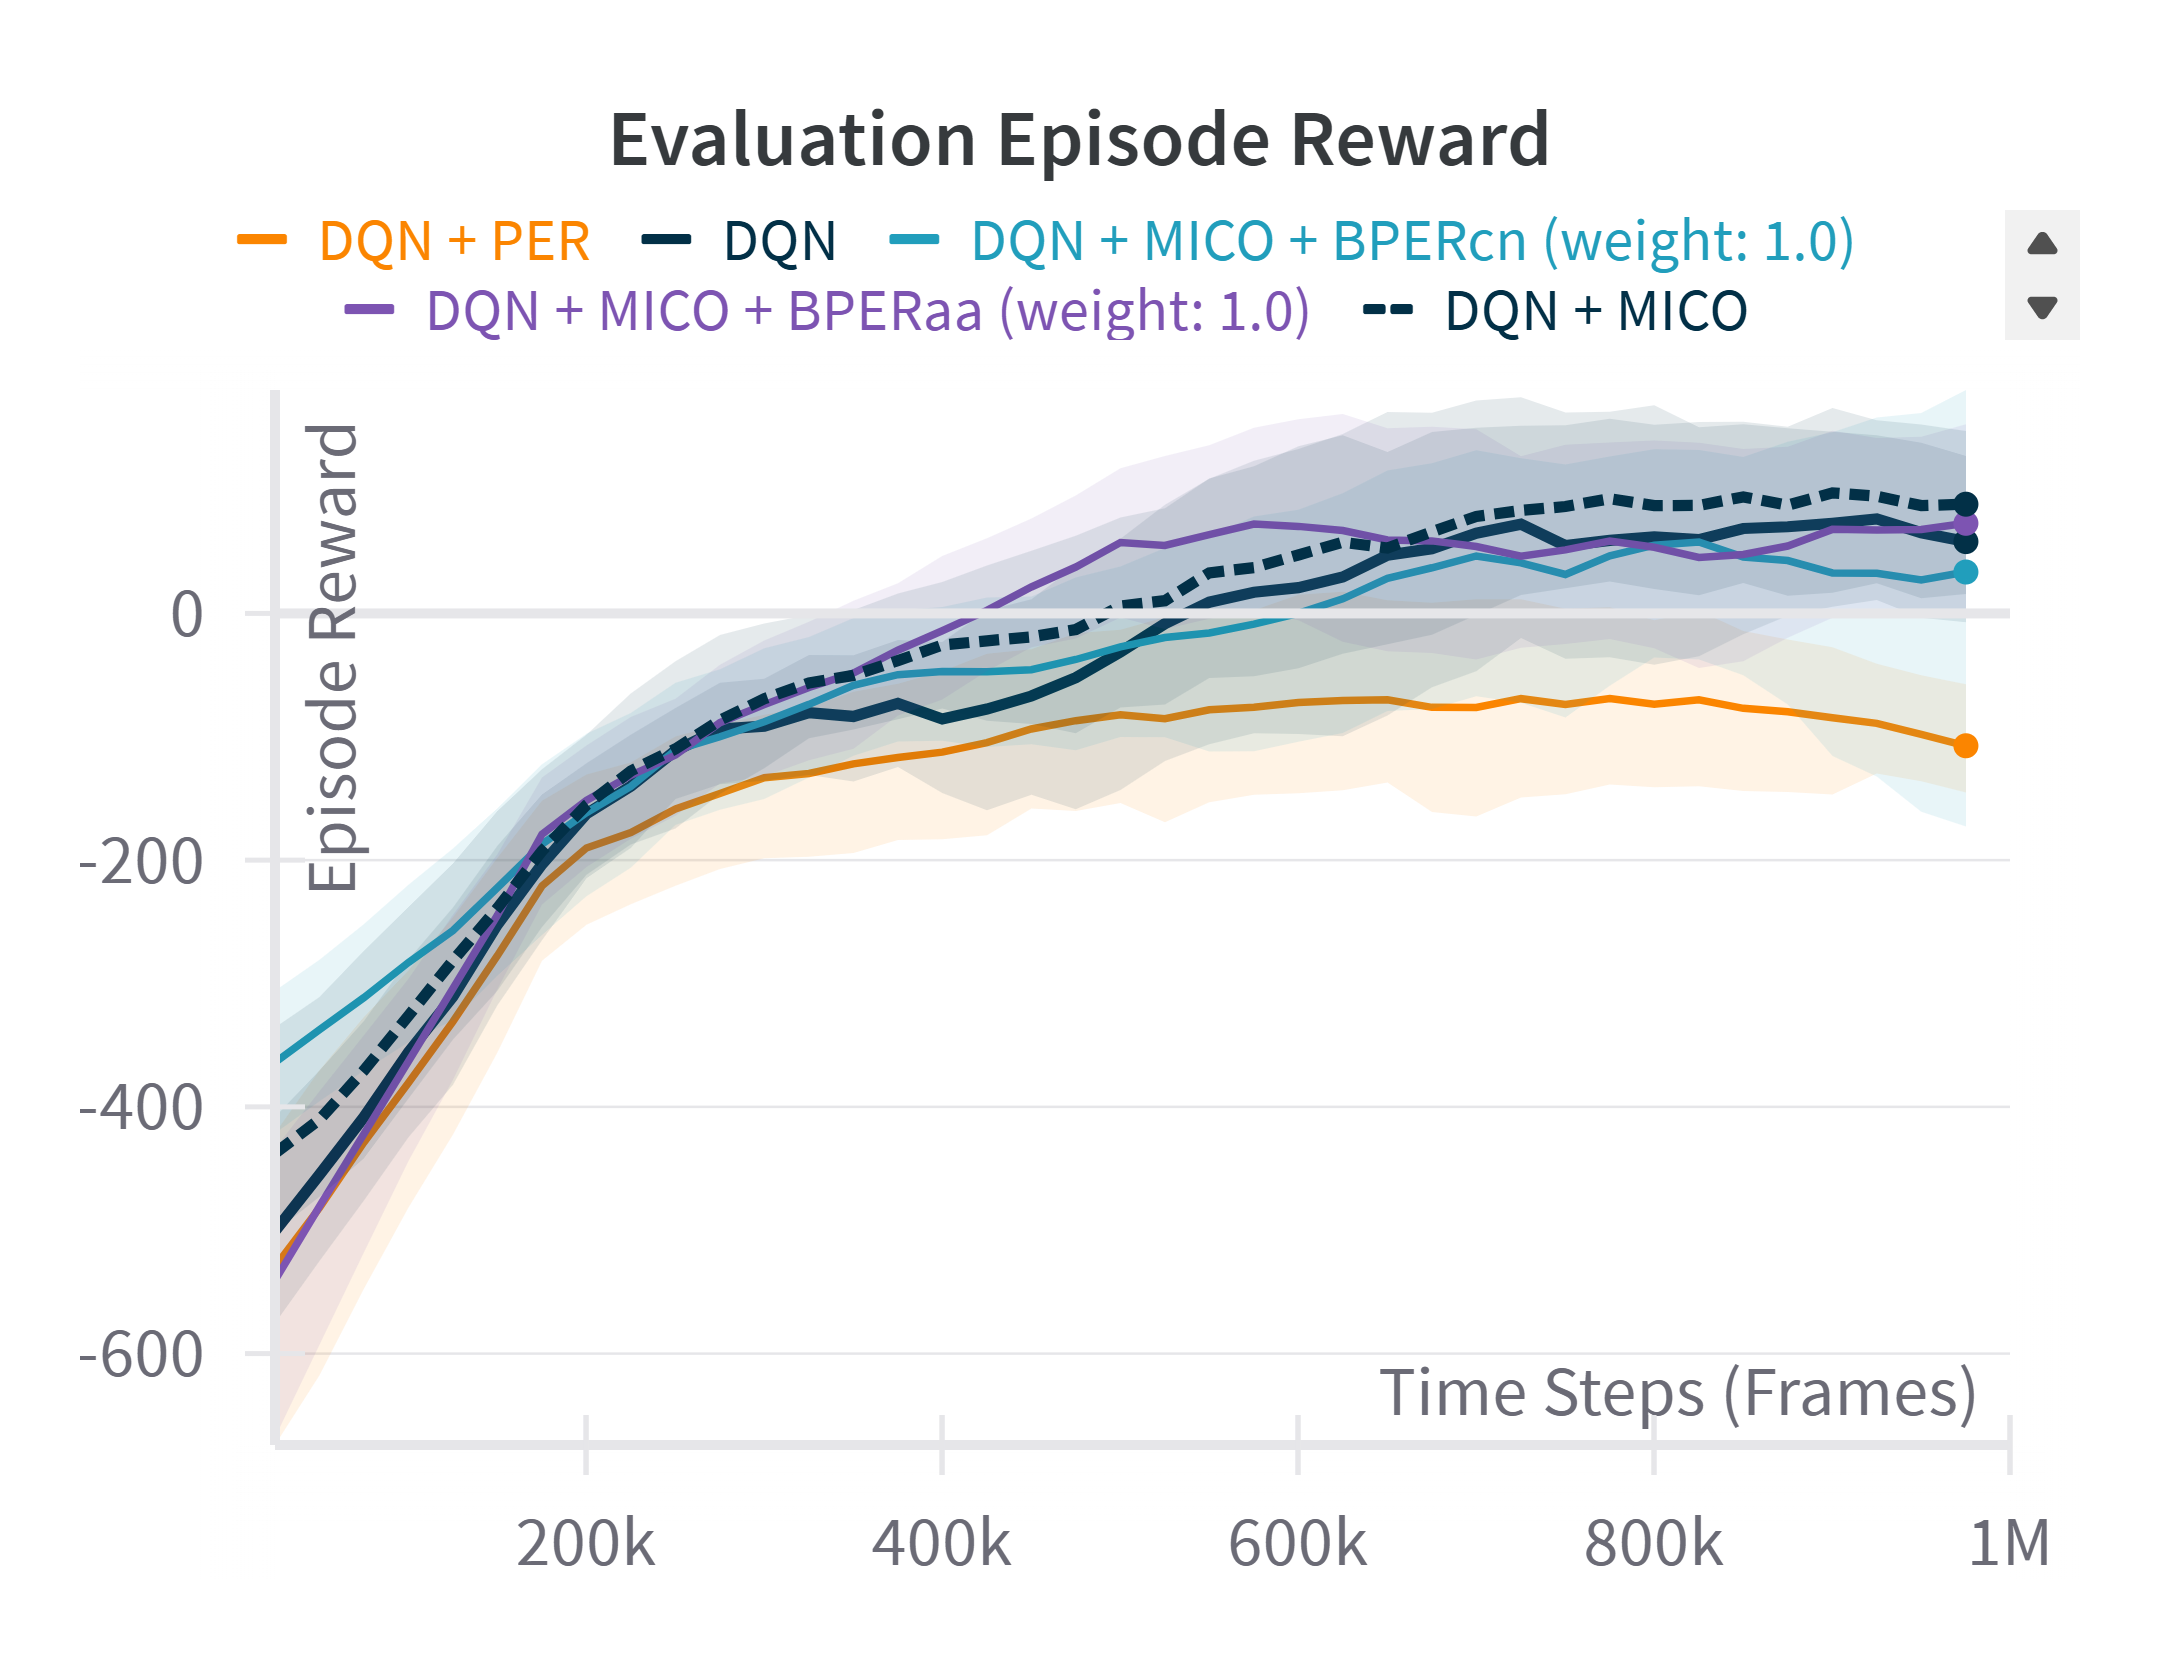
\includegraphics[width=\linewidth]{Results/general_results/eval_return_lunar_lander.png}
%         \caption{LunarLander-v1}
%         \label{fig:eval_return_lunar_lander}
%     \end{subfigure}
%     \hfill
%     \begin{subfigure}{0.45\textwidth}
%         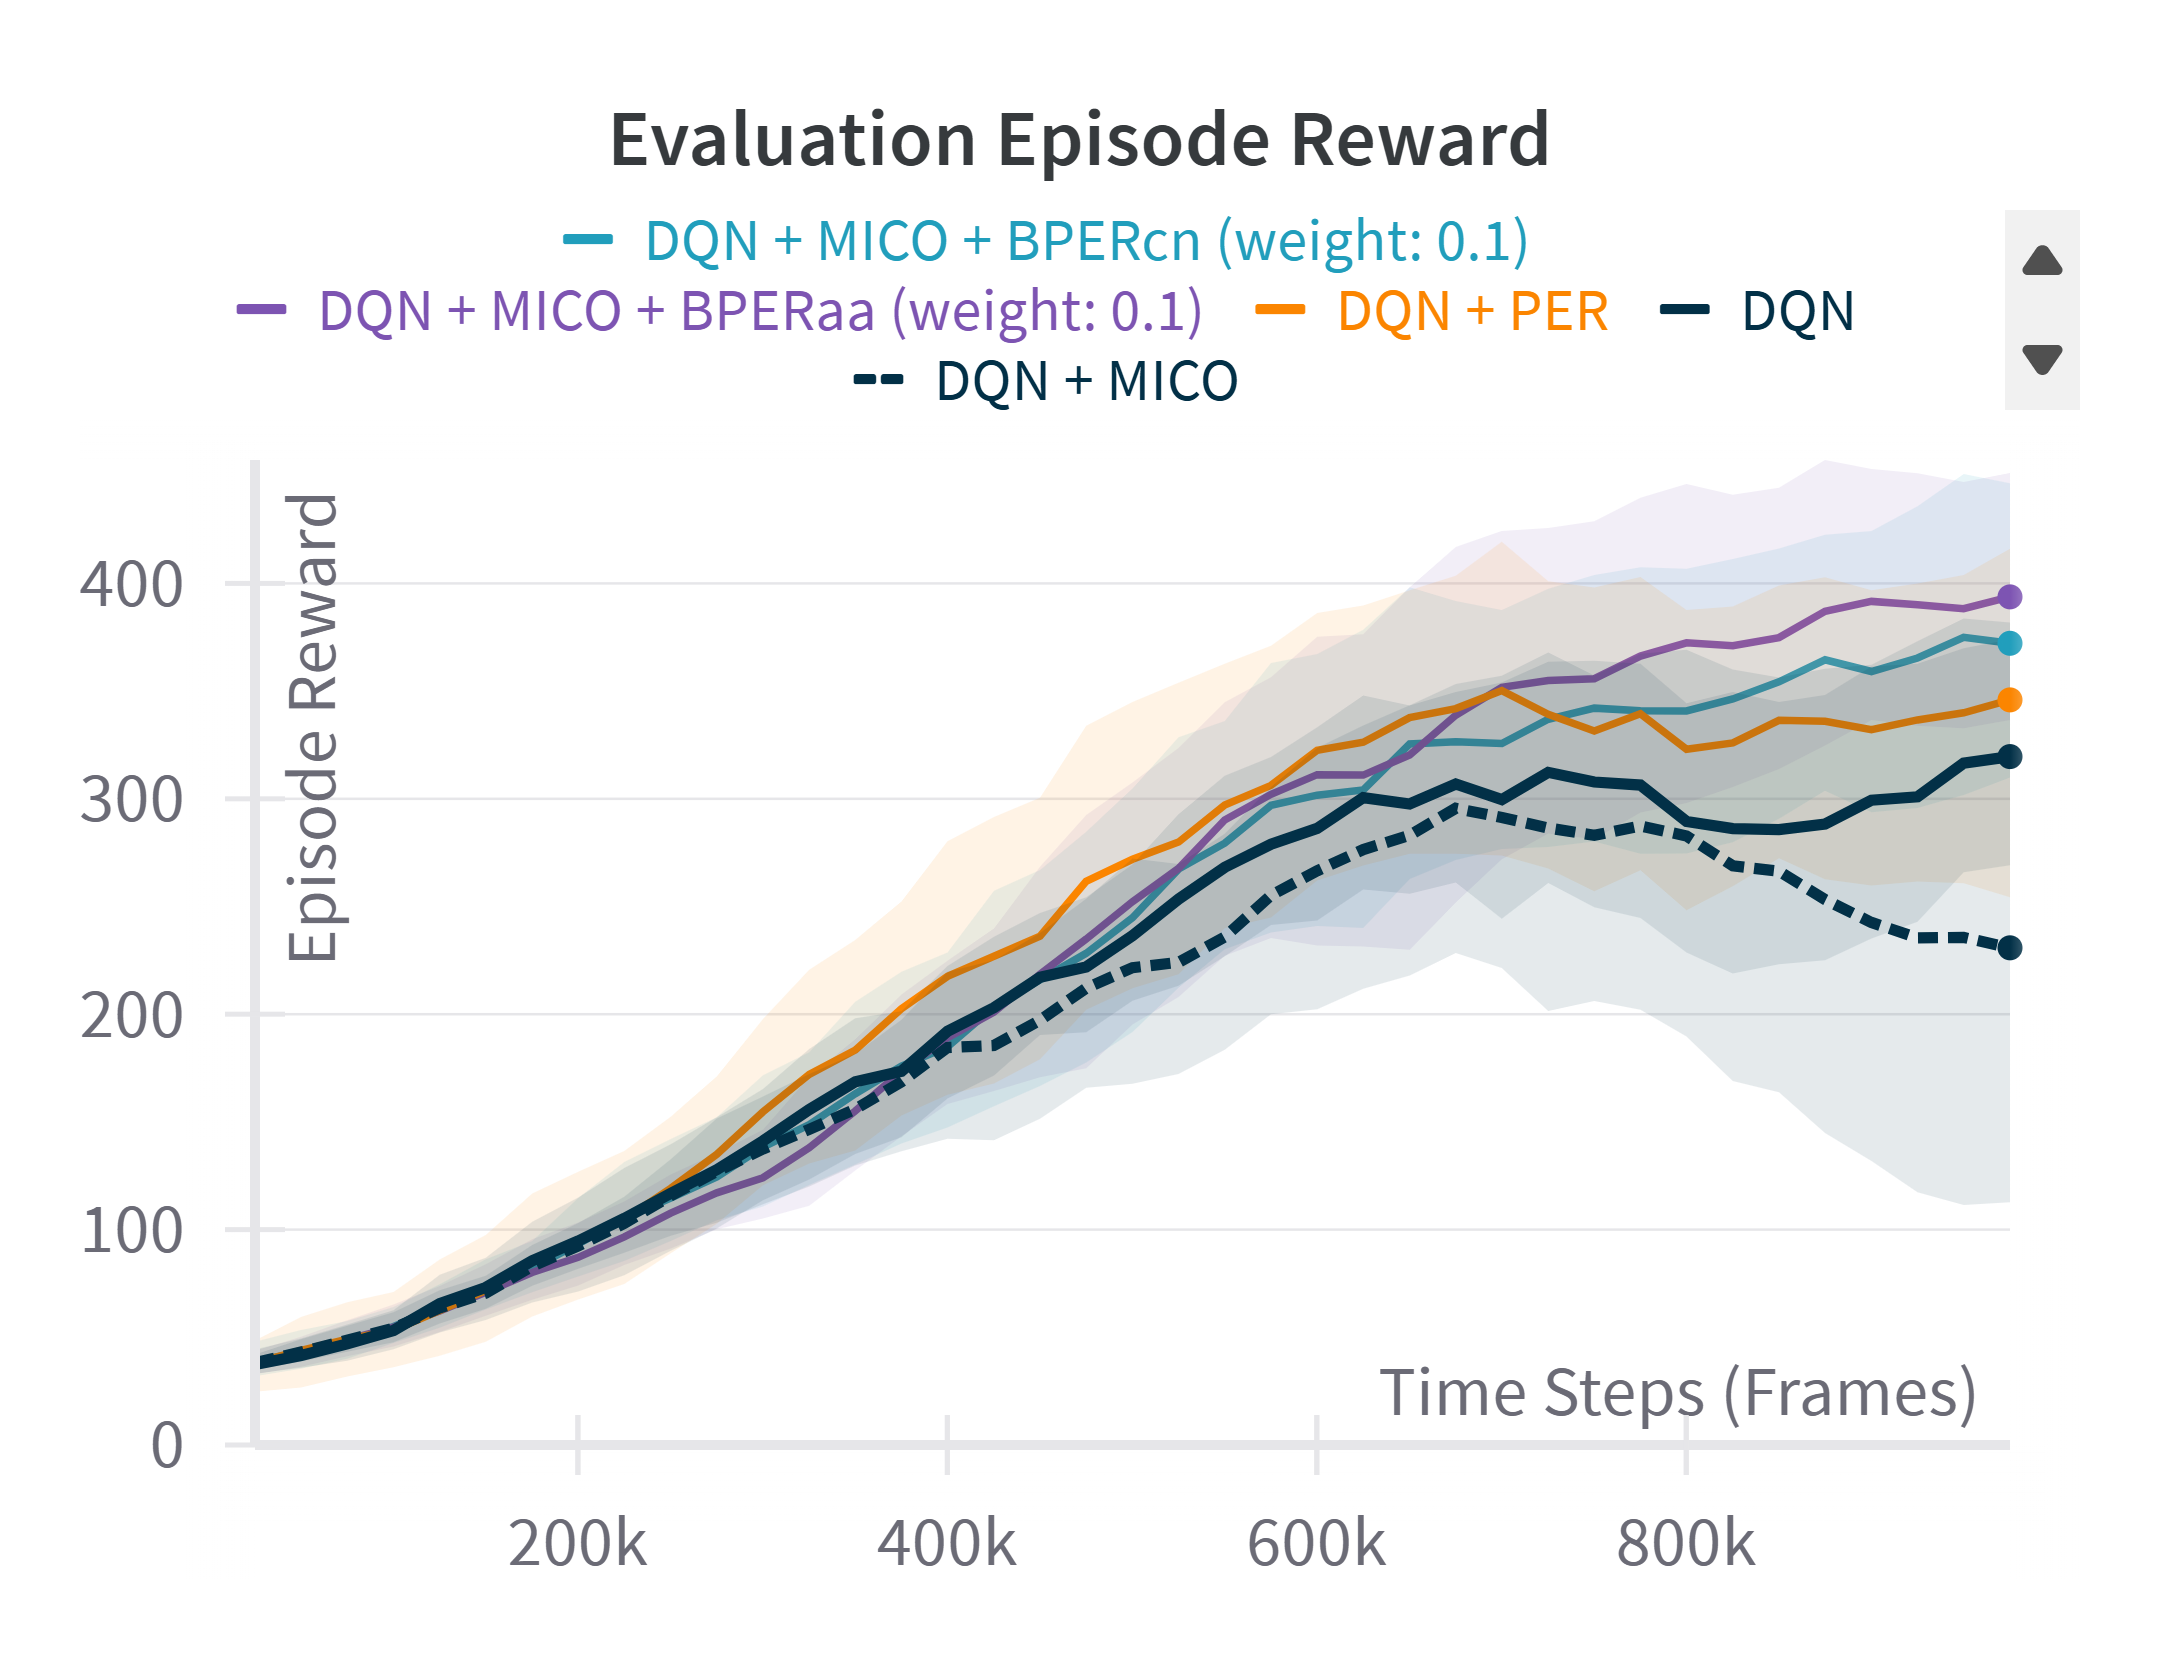
\includegraphics[width=\linewidth]{Results/general_results/eval_return_cartpole_v1.png}
%         \caption{CartPole-v1}
%         \label{fig:eval_return_cartpole_v1}
%     \end{subfigure}
%     \hfill
%     \begin{subfigure}{0.45\textwidth}
%         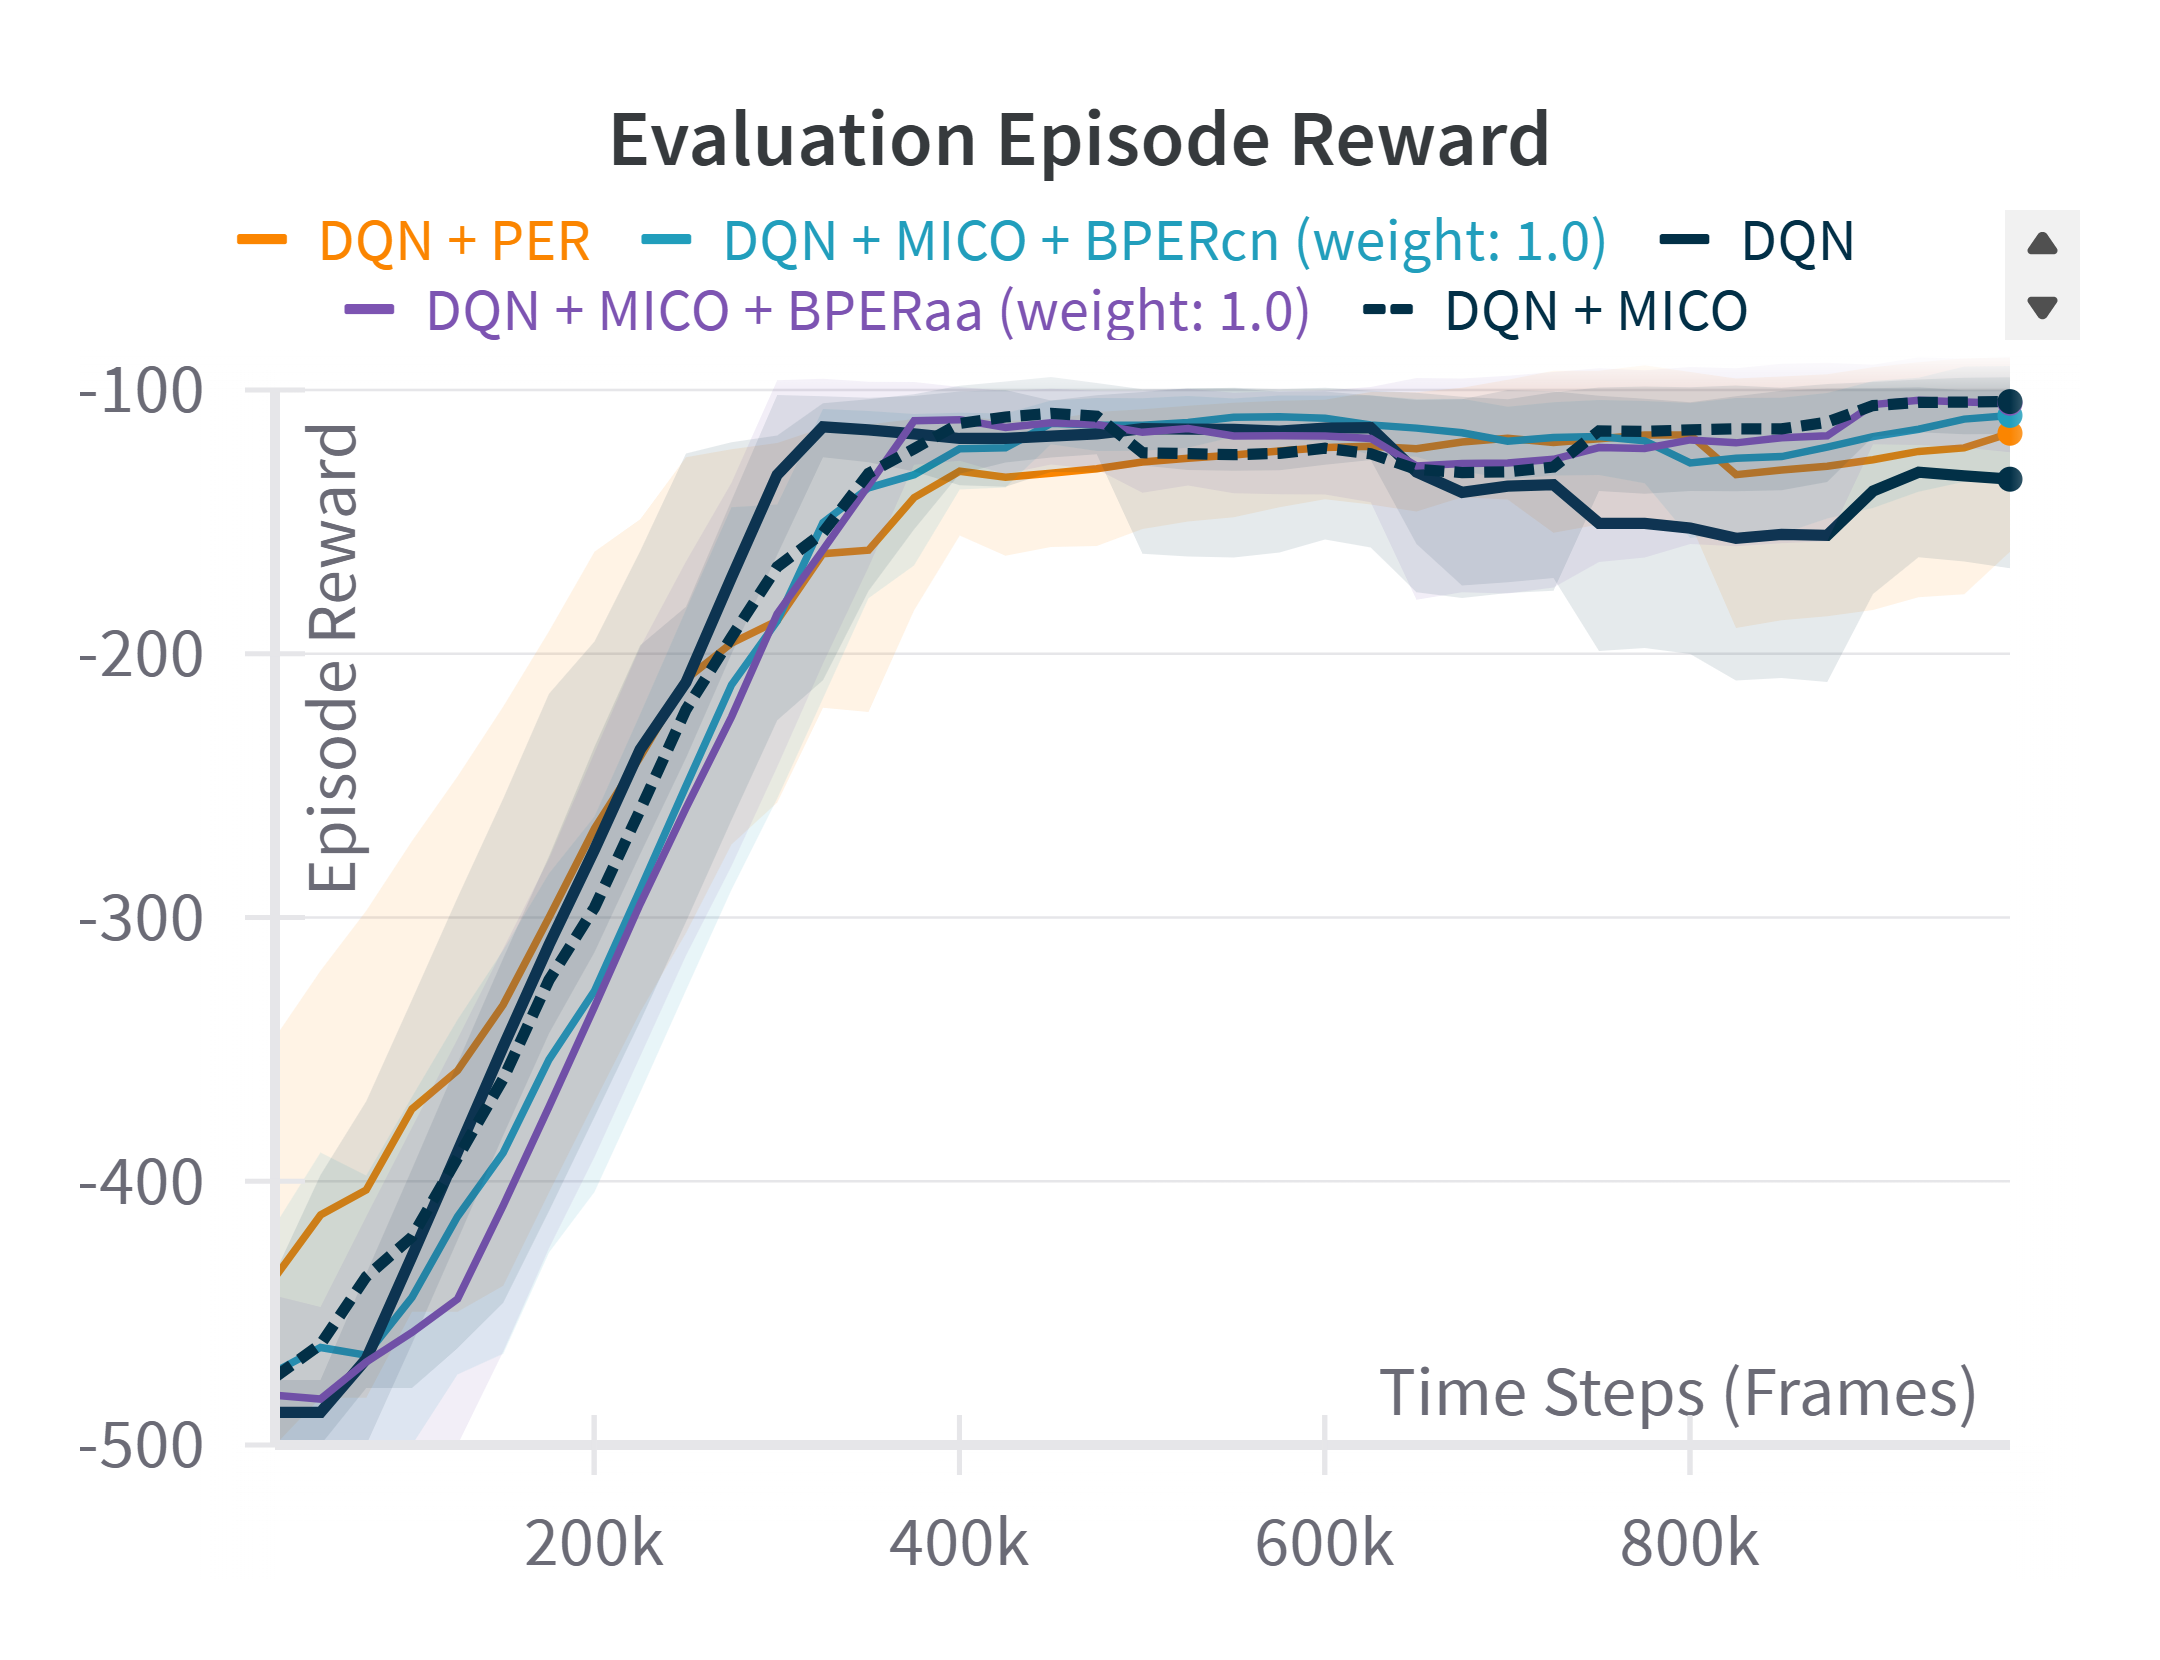
\includegraphics[width=\linewidth]{Results/general_results/eval_return_acrobot.png}
%         \caption{Acrobot-v1}
%         \label{fig:eval_return_acrobot}
%     \end{subfigure}
%     \caption[Validation Episode Reward in Classical Environments]{\textbf{Validation Episode Reward in Classical Environments.} Validation episode reward performance over time, averaged with a moving window of 100 episodes across 5 independent executions, with shaded regions representing the variability for each method. The values are calculated in four different environments: (a) MountainCar-v0, (b) LunarLander-v1, (c) CartPole-v1, and (d) Acrobot-v1.}
%     \label{fig:episode_reward_evaluation}
% \end{figure}



% \newpage
% \section{Episode Reward Gain baseline DQN + MICO}
% \label{append:episode_reward_gain_dqn_mico}

% \begin{figure}[h]
%     \centering
%     \begin{subfigure}{0.45\textwidth}
%     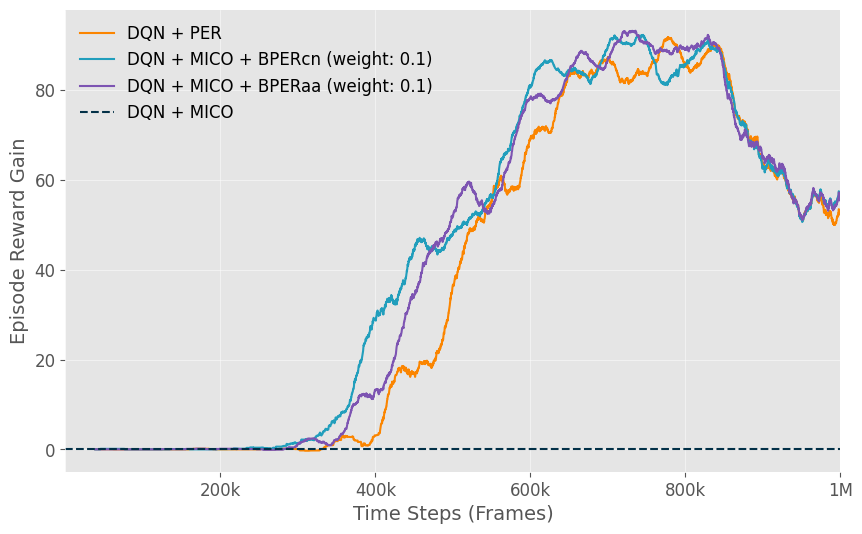
\includegraphics[width=\linewidth]{Results/general_results/mountain_car_reward_gain_vs_dqn_mico.png}
%         \caption{MountainCar-v0}
%         \label{fig:mountain_car_reward_gain_vs_dqn_mico}
%     \end{subfigure}
%     \hfill
%     \begin{subfigure}{0.45\textwidth}
%         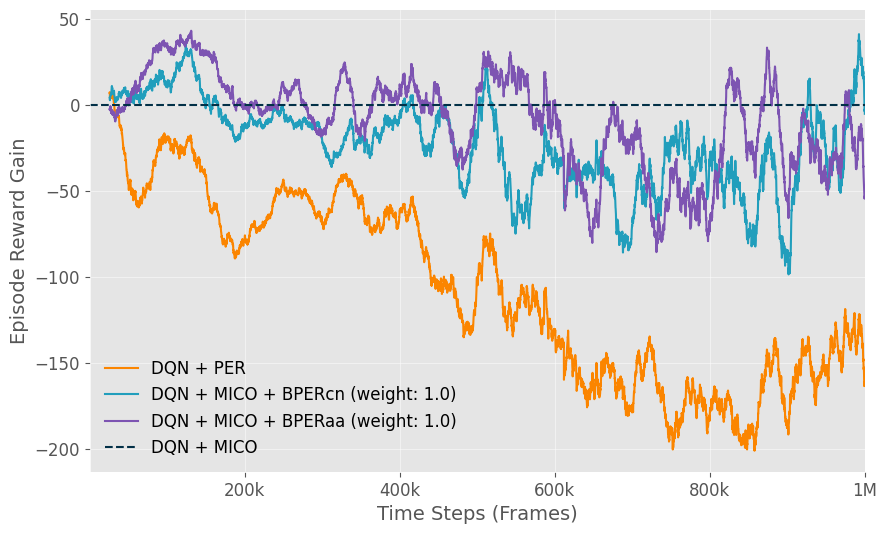
\includegraphics[width=\linewidth]{Results/general_results/lunarlander_reward_gain_vs_dqn_mico.png}
%         \caption{LunarLander-v1}
%         \label{fig:lunarlander_reward_gain_vs_dqn_mico}
%     \end{subfigure}
%     \hfill
%     \begin{subfigure}{0.45\textwidth}
%         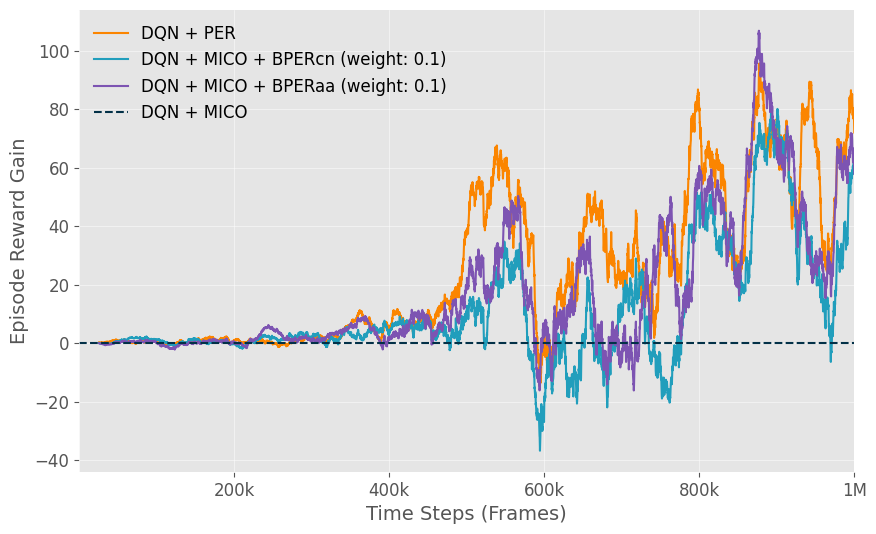
\includegraphics[width=\linewidth]{Results/general_results/cart_polev1_reward_gain_vs_dqn_mico.png}
%         \caption{CartPole-v1}
%         \label{fig:cart_polev1_reward_gain_vs_dqn_mico}
%     \end{subfigure}
%     \hfill
%     \begin{subfigure}{0.45\textwidth}
%         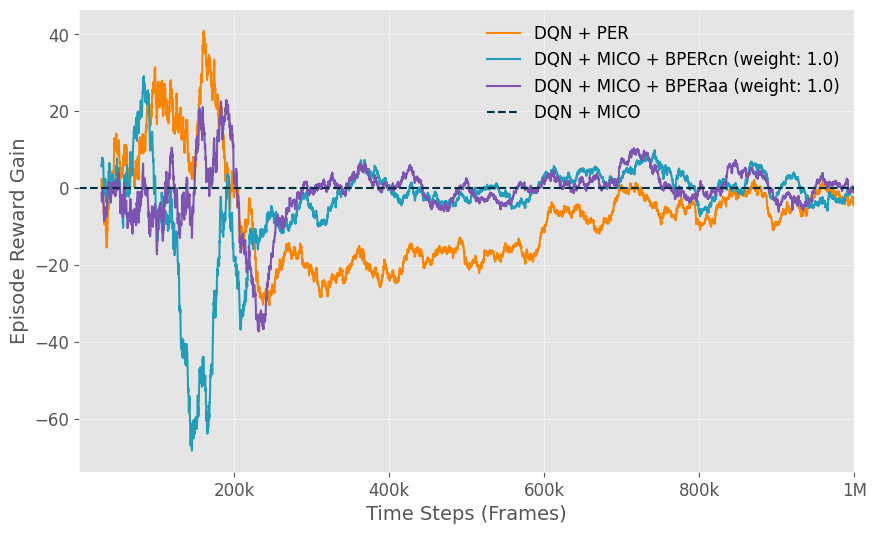
\includegraphics[width=\linewidth]{Results/general_results/acrobotv1_reward_gain_vs_dqn_mico.png}
%         \caption{Acrobot-v1}
%         \label{fig:acrobotv1_reward_gain_vs_dqn_mico}
%     \end{subfigure}
%     \caption[Episode Reward Gain in Classical Environments against DQN MICO baseline]{\textbf{Episode Reward Gain in Classical Environments against DQN MICO baseline.} Episode reward gain performance calculated against the DQN + MICO baseline over time, averaged with a moving window of 100 episodes across 5 independent executions. The values are calculated in four different environments: (a) MountainCar-v0, (b) LunarLander-v1, (c) CartPole-v1, and (d) Acrobot-v1.}
%     \label{fig:reward_gain_vs_dqn_mico_methods}
% \end{figure}

% % \section{Cumulative Reward for Lunar Lander}
% % \label{append:cumulative_reward_lunar_lander}
% % \begin{figure}[H]
% %     \centering
% %     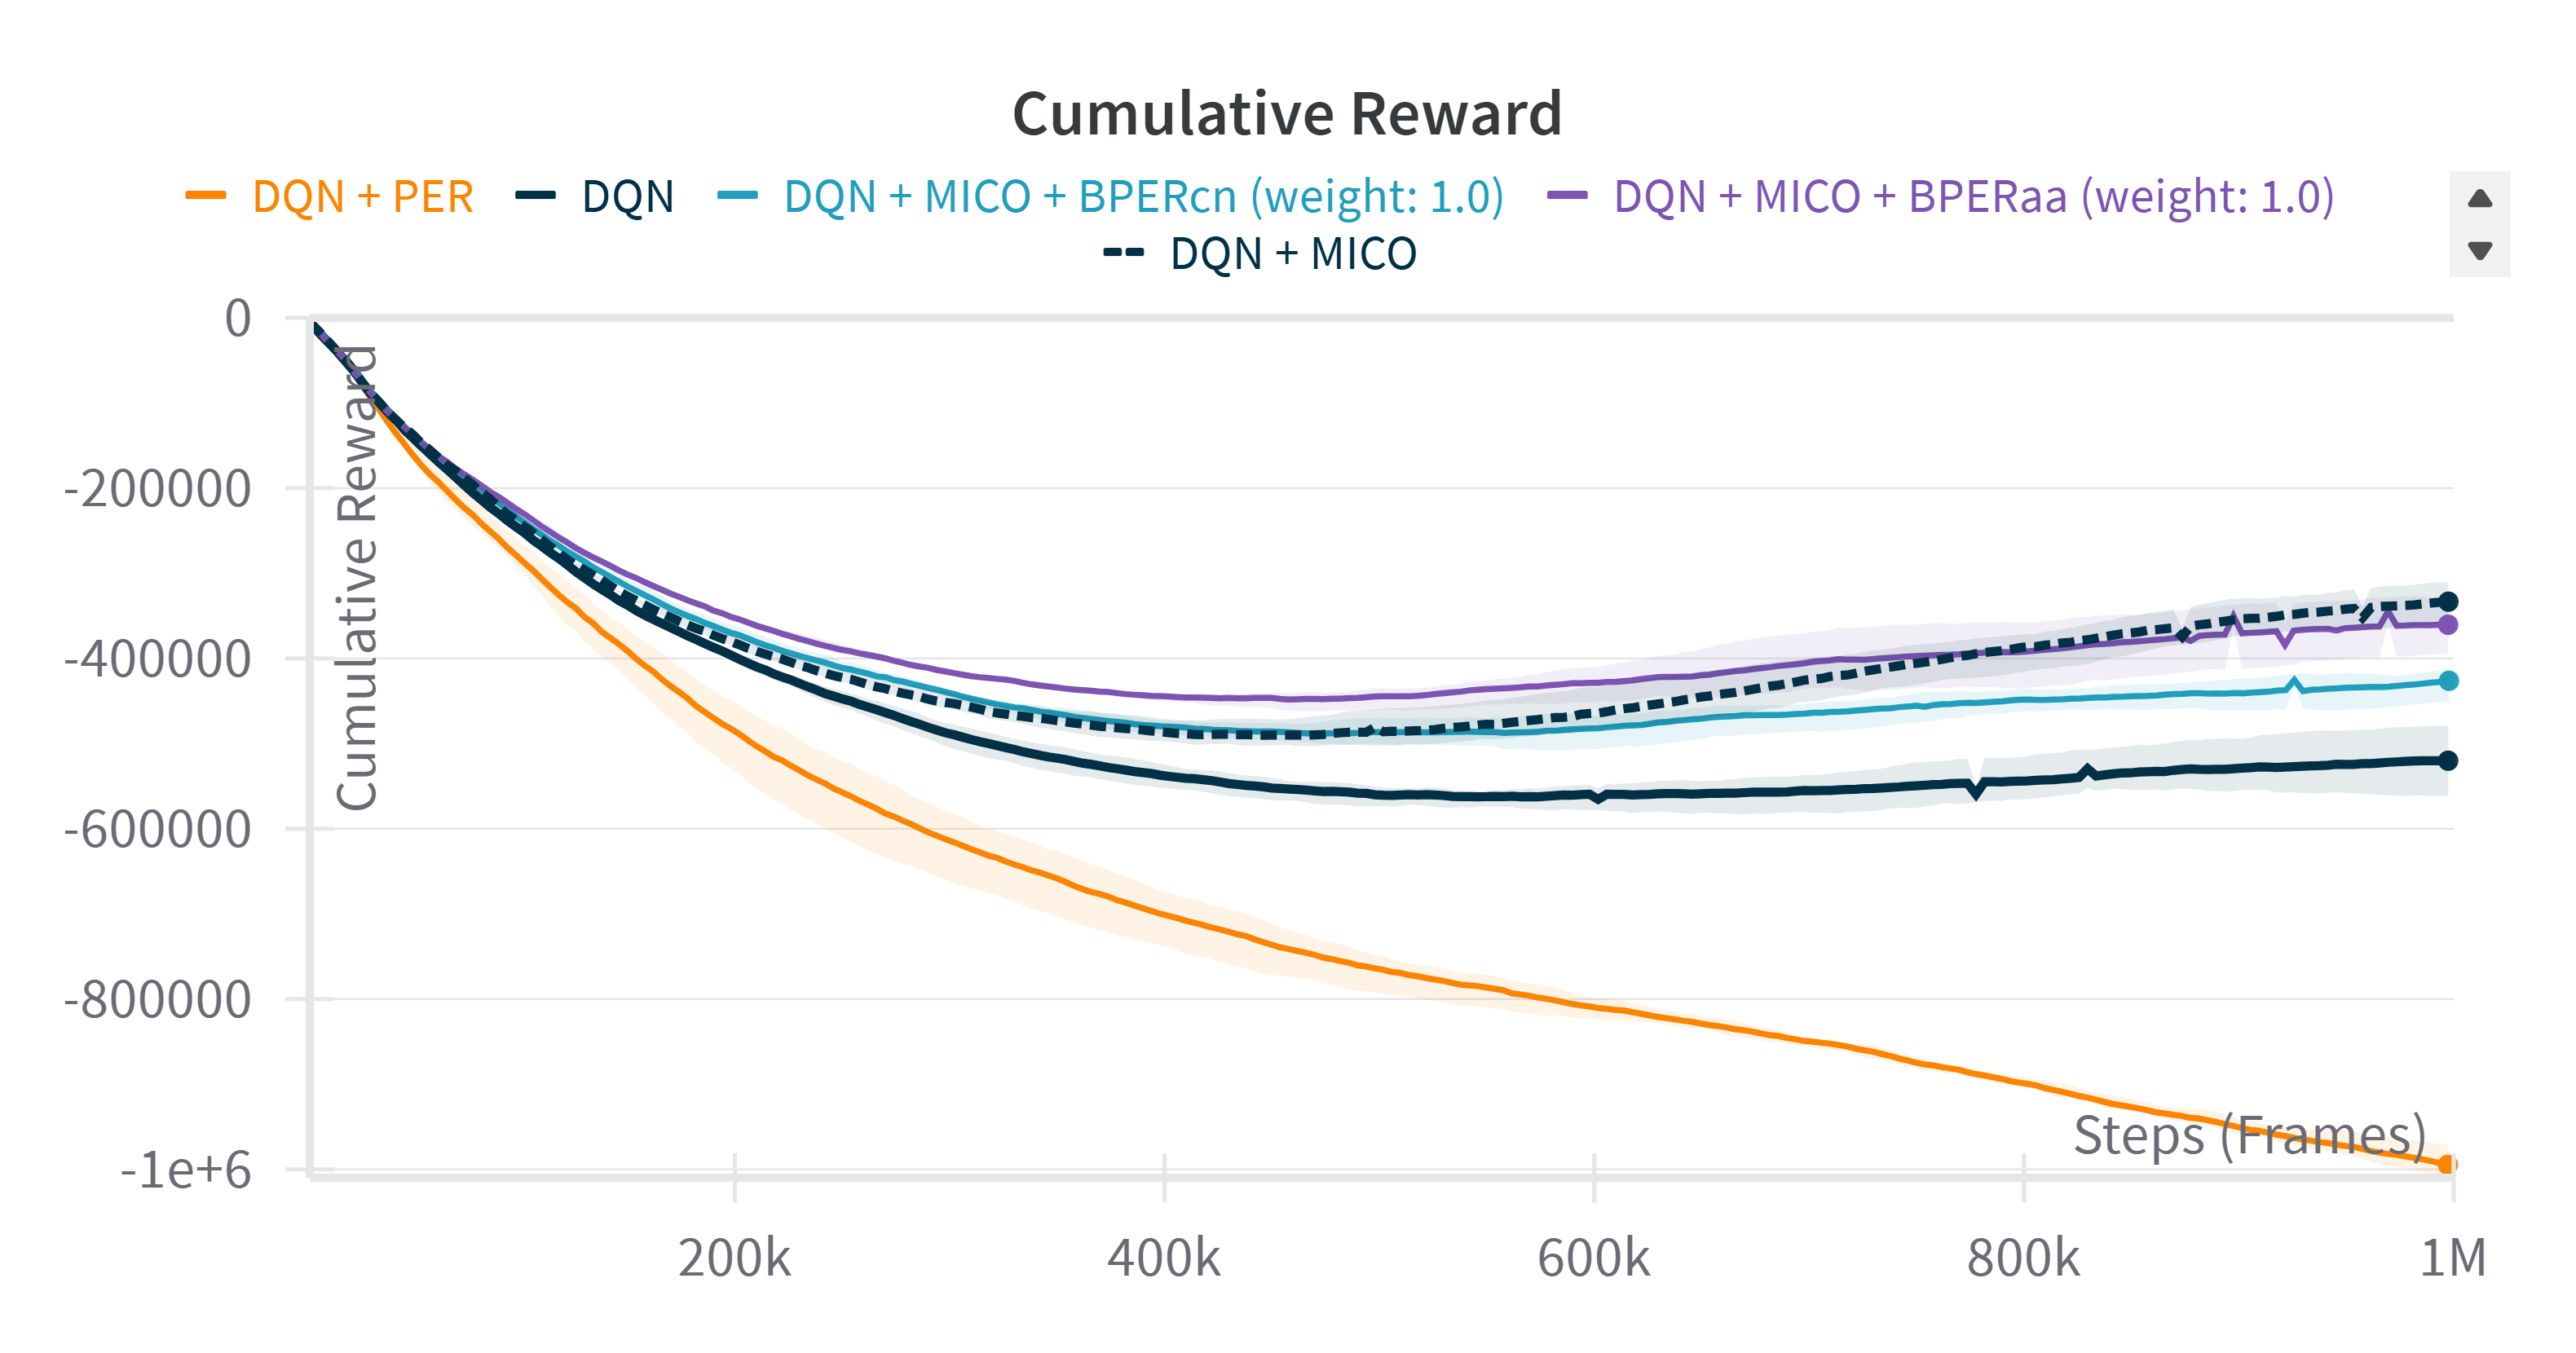
\includegraphics[width=1.\linewidth]{Results/general_results/cumulative_reward_lunar_lander.png}
% %     \caption[Cumulative Reward for Lunar Lander]{\textbf{Cumulative Reward for Lunar Lander}}
% %     \label{fig:cumulative_reward_lunar_lander}
% % \end{figure}

